% Options for packages loaded elsewhere
% Options for packages loaded elsewhere
\PassOptionsToPackage{unicode}{hyperref}
\PassOptionsToPackage{hyphens}{url}
%
\documentclass[
  russian,
  letterpaper,
]{scrbook}
\usepackage{xcolor}
\usepackage{amsmath,amssymb}
\setcounter{secnumdepth}{-\maxdimen} % remove section numbering
\usepackage{iftex}
\ifPDFTeX
  \usepackage[T1]{fontenc}
  \usepackage[utf8]{inputenc}
  \usepackage{textcomp} % provide euro and other symbols
\else % if luatex or xetex
  \usepackage{unicode-math} % this also loads fontspec
  \defaultfontfeatures{Scale=MatchLowercase}
  \defaultfontfeatures[\rmfamily]{Ligatures=TeX,Scale=1}
\fi
\usepackage{lmodern}
\ifPDFTeX\else
  % xetex/luatex font selection
\fi
% Use upquote if available, for straight quotes in verbatim environments
\IfFileExists{upquote.sty}{\usepackage{upquote}}{}
\IfFileExists{microtype.sty}{% use microtype if available
  \usepackage[]{microtype}
  \UseMicrotypeSet[protrusion]{basicmath} % disable protrusion for tt fonts
}{}
\makeatletter
\@ifundefined{KOMAClassName}{% if non-KOMA class
  \IfFileExists{parskip.sty}{%
    \usepackage{parskip}
  }{% else
    \setlength{\parindent}{0pt}
    \setlength{\parskip}{6pt plus 2pt minus 1pt}}
}{% if KOMA class
  \KOMAoptions{parskip=half}}
\makeatother
% Make \paragraph and \subparagraph free-standing
\makeatletter
\ifx\paragraph\undefined\else
  \let\oldparagraph\paragraph
  \renewcommand{\paragraph}{
    \@ifstar
      \xxxParagraphStar
      \xxxParagraphNoStar
  }
  \newcommand{\xxxParagraphStar}[1]{\oldparagraph*{#1}\mbox{}}
  \newcommand{\xxxParagraphNoStar}[1]{\oldparagraph{#1}\mbox{}}
\fi
\ifx\subparagraph\undefined\else
  \let\oldsubparagraph\subparagraph
  \renewcommand{\subparagraph}{
    \@ifstar
      \xxxSubParagraphStar
      \xxxSubParagraphNoStar
  }
  \newcommand{\xxxSubParagraphStar}[1]{\oldsubparagraph*{#1}\mbox{}}
  \newcommand{\xxxSubParagraphNoStar}[1]{\oldsubparagraph{#1}\mbox{}}
\fi
\makeatother

\usepackage{color}
\usepackage{fancyvrb}
\newcommand{\VerbBar}{|}
\newcommand{\VERB}{\Verb[commandchars=\\\{\}]}
\DefineVerbatimEnvironment{Highlighting}{Verbatim}{commandchars=\\\{\}}
% Add ',fontsize=\small' for more characters per line
\usepackage{framed}
\definecolor{shadecolor}{RGB}{241,243,245}
\newenvironment{Shaded}{\begin{snugshade}}{\end{snugshade}}
\newcommand{\AlertTok}[1]{\textcolor[rgb]{0.68,0.00,0.00}{#1}}
\newcommand{\AnnotationTok}[1]{\textcolor[rgb]{0.37,0.37,0.37}{#1}}
\newcommand{\AttributeTok}[1]{\textcolor[rgb]{0.40,0.45,0.13}{#1}}
\newcommand{\BaseNTok}[1]{\textcolor[rgb]{0.68,0.00,0.00}{#1}}
\newcommand{\BuiltInTok}[1]{\textcolor[rgb]{0.00,0.23,0.31}{#1}}
\newcommand{\CharTok}[1]{\textcolor[rgb]{0.13,0.47,0.30}{#1}}
\newcommand{\CommentTok}[1]{\textcolor[rgb]{0.37,0.37,0.37}{#1}}
\newcommand{\CommentVarTok}[1]{\textcolor[rgb]{0.37,0.37,0.37}{\textit{#1}}}
\newcommand{\ConstantTok}[1]{\textcolor[rgb]{0.56,0.35,0.01}{#1}}
\newcommand{\ControlFlowTok}[1]{\textcolor[rgb]{0.00,0.23,0.31}{\textbf{#1}}}
\newcommand{\DataTypeTok}[1]{\textcolor[rgb]{0.68,0.00,0.00}{#1}}
\newcommand{\DecValTok}[1]{\textcolor[rgb]{0.68,0.00,0.00}{#1}}
\newcommand{\DocumentationTok}[1]{\textcolor[rgb]{0.37,0.37,0.37}{\textit{#1}}}
\newcommand{\ErrorTok}[1]{\textcolor[rgb]{0.68,0.00,0.00}{#1}}
\newcommand{\ExtensionTok}[1]{\textcolor[rgb]{0.00,0.23,0.31}{#1}}
\newcommand{\FloatTok}[1]{\textcolor[rgb]{0.68,0.00,0.00}{#1}}
\newcommand{\FunctionTok}[1]{\textcolor[rgb]{0.28,0.35,0.67}{#1}}
\newcommand{\ImportTok}[1]{\textcolor[rgb]{0.00,0.46,0.62}{#1}}
\newcommand{\InformationTok}[1]{\textcolor[rgb]{0.37,0.37,0.37}{#1}}
\newcommand{\KeywordTok}[1]{\textcolor[rgb]{0.00,0.23,0.31}{\textbf{#1}}}
\newcommand{\NormalTok}[1]{\textcolor[rgb]{0.00,0.23,0.31}{#1}}
\newcommand{\OperatorTok}[1]{\textcolor[rgb]{0.37,0.37,0.37}{#1}}
\newcommand{\OtherTok}[1]{\textcolor[rgb]{0.00,0.23,0.31}{#1}}
\newcommand{\PreprocessorTok}[1]{\textcolor[rgb]{0.68,0.00,0.00}{#1}}
\newcommand{\RegionMarkerTok}[1]{\textcolor[rgb]{0.00,0.23,0.31}{#1}}
\newcommand{\SpecialCharTok}[1]{\textcolor[rgb]{0.37,0.37,0.37}{#1}}
\newcommand{\SpecialStringTok}[1]{\textcolor[rgb]{0.13,0.47,0.30}{#1}}
\newcommand{\StringTok}[1]{\textcolor[rgb]{0.13,0.47,0.30}{#1}}
\newcommand{\VariableTok}[1]{\textcolor[rgb]{0.07,0.07,0.07}{#1}}
\newcommand{\VerbatimStringTok}[1]{\textcolor[rgb]{0.13,0.47,0.30}{#1}}
\newcommand{\WarningTok}[1]{\textcolor[rgb]{0.37,0.37,0.37}{\textit{#1}}}

\usepackage{longtable,booktabs,array}
\newcounter{none} % for unnumbered tables
\usepackage{calc} % for calculating minipage widths
% Correct order of tables after \paragraph or \subparagraph
\usepackage{etoolbox}
\makeatletter
\patchcmd\longtable{\par}{\if@noskipsec\mbox{}\fi\par}{}{}
\makeatother
% Allow footnotes in longtable head/foot
\IfFileExists{footnotehyper.sty}{\usepackage{footnotehyper}}{\usepackage{footnote}}
\makesavenoteenv{longtable}
\usepackage{graphicx}
\makeatletter
\newsavebox\pandoc@box
\newcommand*\pandocbounded[1]{% scales image to fit in text height/width
  \sbox\pandoc@box{#1}%
  \Gscale@div\@tempa{\textheight}{\dimexpr\ht\pandoc@box+\dp\pandoc@box\relax}%
  \Gscale@div\@tempb{\linewidth}{\wd\pandoc@box}%
  \ifdim\@tempb\p@<\@tempa\p@\let\@tempa\@tempb\fi% select the smaller of both
  \ifdim\@tempa\p@<\p@\scalebox{\@tempa}{\usebox\pandoc@box}%
  \else\usebox{\pandoc@box}%
  \fi%
}
% Set default figure placement to htbp
\def\fps@figure{htbp}
\makeatother



\ifLuaTeX
\usepackage[bidi=basic,shorthands=off,provide=*]{babel}
\else
\usepackage[bidi=default,shorthands=off,provide=*]{babel}
\fi
\ifLuaTeX
  \usepackage{selnolig} % disable illegal ligatures
\fi


\setlength{\emergencystretch}{3em} % prevent overfull lines

\providecommand{\tightlist}{%
  \setlength{\itemsep}{0pt}\setlength{\parskip}{0pt}}



 


\usepackage{fontspec}
\usepackage{polyglossia}
\usepackage{unicode-math}
\usepackage{amsmath}
\usepackage{mathtools}
\usepackage{graphicx}
\usepackage{float}
\usepackage{booktabs}
\usepackage{longtable}
\usepackage{array}
\usepackage{microtype}
\usepackage{hyperref}

\defaultfontfeatures{Ligatures=TeX, Scale=MatchLowercase}
\setmainfont{Libertinus Serif}
\setsansfont{Libertinus Sans}
\setmonofont{Libertinus Mono}[Scale=0.9]
\setmathfont{Libertinus Math}

\setlength{\emergencystretch}{3em}

\hypersetup{
  pdfborder={0 0 0},
  colorlinks=true,
  linkcolor=black,
  citecolor=black,
  urlcolor=black
}

\newcommand{\E}{\mathbb{E}}
\newcommand{\Var}{\operatorname{Var}}
\newcommand{\cov}{\operatorname{cov}}
\newcommand{\dd}{\,\mathrm{d}}
\setmainlanguage{russian}
\setotherlanguage{english}
\PolyglossiaSetup{russian}{
  bcp47=ru,
  scripttag=cyrl,
  langtag=RUS,
  hyphennames={russian},
  hyphenmins={2,2},
  frenchspacing=true,
  indentfirst=true
}
\makeatletter
\@ifpackageloaded{bookmark}{}{\usepackage{bookmark}}
\makeatother
\makeatletter
\@ifpackageloaded{caption}{}{\usepackage{caption}}
\AtBeginDocument{%
\ifdefined\contentsname
  \renewcommand*\contentsname{Содержание}
\else
  \newcommand\contentsname{Содержание}
\fi
\ifdefined\listfigurename
  \renewcommand*\listfigurename{Список Иллюстраций}
\else
  \newcommand\listfigurename{Список Иллюстраций}
\fi
\ifdefined\listtablename
  \renewcommand*\listtablename{Список Таблиц}
\else
  \newcommand\listtablename{Список Таблиц}
\fi
\ifdefined\figurename
  \renewcommand*\figurename{Рисунок}
\else
  \newcommand\figurename{Рисунок}
\fi
\ifdefined\tablename
  \renewcommand*\tablename{Таблица}
\else
  \newcommand\tablename{Таблица}
\fi
}
\@ifpackageloaded{float}{}{\usepackage{float}}
\floatstyle{ruled}
\@ifundefined{c@chapter}{\newfloat{codelisting}{h}{lop}}{\newfloat{codelisting}{h}{lop}[chapter]}
\floatname{codelisting}{Список}
\newcommand*\listoflistings{\listof{codelisting}{Список Каталогов}}
\makeatother
\makeatletter
\makeatother
\makeatletter
\@ifpackageloaded{caption}{}{\usepackage{caption}}
\@ifpackageloaded{subcaption}{}{\usepackage{subcaption}}
\makeatother
\usepackage{bookmark}
\IfFileExists{xurl.sty}{\usepackage{xurl}}{} % add URL line breaks if available
\urlstyle{same}
\hypersetup{
  pdftitle={Статистический анализ данных},
  pdfauthor={Дмитрий В. Наумов},
  pdflang={ru},
  hidelinks,
  pdfcreator={LaTeX via pandoc}}


\title{Статистический анализ данных}
\usepackage{etoolbox}
\makeatletter
\providecommand{\subtitle}[1]{% add subtitle to \maketitle
  \apptocmd{\@title}{\par {\large #1 \par}}{}{}
}
\makeatother
\subtitle{От вероятности к физическому результату}
\author{Дмитрий В. Наумов}
\date{}
\begin{document}
\frontmatter
\maketitle


\mainmatter
\bookmarksetup{startatroot}

\chapter*{Статистический анализ
данных}\label{ux441ux442ux430ux442ux438ux441ux442ux438ux447ux435ux441ux43aux438ux439-ux430ux43dux430ux43bux438ux437-ux434ux430ux43dux43dux44bux445}
\addcontentsline{toc}{chapter}{Статистический анализ данных}

\markboth{Статистический анализ данных}{Статистический анализ данных}

\section*{Как читать эту
книгу}\label{ux43aux430ux43a-ux447ux438ux442ux430ux442ux44c-ux44dux442ux443-ux43aux43dux438ux433ux443}
\addcontentsline{toc}{section}{Как читать эту книгу}

\markright{Как читать эту книгу}

Книга следует естественной логике анализа данных: от языка вероятностей
и случайных величин к оцениванию параметров, проверке гипотез и
полноценному экспериментальному результату. Материал можно читать
последовательно или использовать как справочник.

\textbf{Статус проекта.} Это живая онлайн-книга. Текст, интерактивы и
примеры будут уточняться вместе с развитием курса.

\bookmarksetup{startatroot}

\chapter*{Предисловие}\label{ux43fux440ux435ux434ux438ux441ux43bux43eux432ux438ux435}
\addcontentsline{toc}{chapter}{Предисловие}

\markboth{Предисловие}{Предисловие}

Современный эксперимент практически невозможен без статистического
анализа данных. От выбора функции правдоподобия, корректного учёта фона
и систематических неопределённостей, построения доверительных интервалов
и проверки гипотез напрямую зависит физический результат. Поэтому
статистика в экспериментальной физике --- не вспомогательный раздел, а
один из основных рабочих инструментов исследователя.

Этот курс посвящён именно тем методам статистического анализа, которые
действительно нужны на практике. Он основан на личном опыте автора,
накопленном за три десятилетия работы с экспериментальными данными в
физике элементарных частиц, нейтринной физике и астрофизике. Здесь
изложено не всё, что можно найти в обширной литературе по математической
статистике, а прежде всего то, что регулярно используется в реальном
анализе данных и помогает получать надёжные, физически осмысленные
результаты.

Основная цель курса --- дать читателю не только набор формул и
алгоритмов, но и понимание того, как мыслить статистически в контексте
эксперимента. Поэтому в книге сочетаются теоретическое изложение, разбор
типичных задач и большое количество примеров, включая вычисления и код
на Python в ноутбуках. Такой формат позволяет не просто прочитать
материал, но и сразу воспроизвести ключевые результаты, проверить их на
игрушечных моделях и использовать как основу для собственной работы.

При изложении я стремился к простоте, ясности и практической
направленности. По возможности обсуждаются физический смысл методов,
область их применимости, типичные ошибки и ограничения. Особое внимание
уделено тем вопросам, с которыми студент, аспирант или молодой
исследователь действительно сталкивается при анализе экспериментальных
данных.

Курс создан в рамках программы «Физика нейтрино и астрофизика», однако
его содержание значительно шире и может быть полезно всем, кто
занимается экспериментальной физикой и обработкой данных. Он рассчитан
на студентов старших курсов, аспирантов и исследователей, уже знакомых с
основами теории вероятностей, математического анализа и программирования
на Python.

Я надеюсь, что этот курс поможет читателю перейти от формального
знакомства со статистическими методами к их уверенному и осмысленному
применению в реальной научной работе.

\bookmarksetup{startatroot}

\chapter*{Маршрут
книги}\label{ux43cux430ux440ux448ux440ux443ux442-ux43aux43dux438ux433ux438}
\addcontentsline{toc}{chapter}{Маршрут книги}

\markboth{Маршрут книги}{Маршрут книги}

Книга строится не как энциклопедия формул, а как последовательный путь
от физического вопроса к статистическому выводу.

\section*{Шестнадцать
глав}\label{ux448ux435ux441ux442ux43dux430ux434ux446ux430ux442ux44c-ux433ux43bux430ux432}
\addcontentsline{toc}{section}{Шестнадцать глав}

\markright{Шестнадцать глав}

{\def\LTcaptype{none} % do not increment counter
\begin{longtable}[]{@{}
  >{\raggedleft\arraybackslash}p{(\linewidth - 4\tabcolsep) * \real{0.4000}}
  >{\raggedright\arraybackslash}p{(\linewidth - 4\tabcolsep) * \real{0.3000}}
  >{\raggedright\arraybackslash}p{(\linewidth - 4\tabcolsep) * \real{0.3000}}@{}}
\toprule\noalign{}
\begin{minipage}[b]{\linewidth}\raggedleft
№
\end{minipage} & \begin{minipage}[b]{\linewidth}\raggedright
Глава
\end{minipage} & \begin{minipage}[b]{\linewidth}\raggedright
Статус
\end{minipage} \\
\midrule\noalign{}
\endhead
\bottomrule\noalign{}
\endlastfoot
1 & \href{chapters/why_statistics.qmd}{Зачем физику статистика} & Первая
редакция \\
2 & \href{chapters/01_random_distributions.qmd}{Случайные величины,
распределения, моменты} & Заготовка \\
3 & \href{chapters/02_characteristic_functions.qmd}{Характеристические
функции и суммы случайных величин} & Заготовка \\
4 & \href{chapters/03_central_limit_theorem.qmd}{Центральная предельная
теорема и нормальное распределение} & Заготовка \\
5 & \href{chapters/04_non_gaussian_clt_violations.qmd}{Когда не
возникает гауссового распределения} & Заготовка \\
6 &
\href{chapters/05_error_propagation_and_covariance.qmd}{Распространение
ошибок, ковариации и многомерный гаусс} & Заготовка \\
7 & \href{chapters/06_monte_carlo_method.qmd}{Метод Монте-Карло и
псевдоэксперименты} & Заготовка \\
8 &
\href{chapters/07_parameter_estimation_and_maximum_likelihood.qmd}{Оценивание
параметров и метод максимального правдоподобия} & Заготовка \\
9 & \href{chapters/08_method_of_least_squares.qmd}{Метод наименьших
квадратов} & Заготовка \\
10 & \href{chapters/09_statistical_tests_basics.qmd}{Статистические
тесты: общие понятия} & Заготовка \\
11 &
\href{chapters/10_test_statistics_and_multivariate_methods.qmd}{Статистики
тестов и многомерные методы} & Заготовка \\
12 & \href{chapters/11_goodness_of_fit_and_significance.qmd}{Проверка
согласия и статистическая значимость} & Заготовка \\
13 & \href{chapters/12_feldman_cousins_and_cls.qmd}{Фельдман--Казинс,
CLs и родственные методы} & Заготовка \\
14 & \href{chapters/13_interval_estimation_and_limits.qmd}{Интервальные
оценки и установление ограничений} & Заготовка \\
15 &
\href{chapters/14_nuisance_parameters_and_systematics.qmd}{Nuisance-параметры
и систематические неопределённости} & Заготовка \\
16 & \href{chapters/15_bayesian_examples.qmd}{Байесовский вывод и
практические примеры} & Заготовка \\
\end{longtable}
}

\part{I. Вероятностный язык}

\chapter{Зачем физику
статистика}\label{ux437ux430ux447ux435ux43c-ux444ux438ux437ux438ux43aux443-ux441ux442ux430ux442ux438ux441ux442ux438ux43aux430}

Статистика в экспериментальной физике нужна не после измерения, а на
каждом его этапе. Она связывает теоретическое предсказание, устройство
эксперимента, наблюдённые данные и формулировку результата.

{Главная мысль}

Эксперимент даёт не готовый ответ, а данные, подверженные случайным
флуктуациям. Чтобы превратить их в физический вывод, нужна явно
сформулированная статистическая модель.

После этой главы читатель сможет:

\begin{itemize}
\tightlist
\item
  различать теоретическое предсказание, наблюдение и статистический
  вывод;
\item
  читать основные формулировки экспериментальных результатов;
\item
  понимать разницу между частотной и байесовской интерпретациями
  вероятности;
\item
  различать параметр модели и его оценку;
\item
  проследить полный путь от псевдоданных до простейшего фита.
\end{itemize}

\section{От физического вопроса к
статье}\label{ux43eux442-ux444ux438ux437ux438ux447ux435ux441ux43aux43eux433ux43e-ux432ux43eux43fux440ux43eux441ux430-ux43a-ux441ux442ux430ux442ux44cux435}

Большинство экспериментальных исследований можно представить как четыре
последовательных шага.

Теоретическая модель редко предсказывает единственное число. Обычно она
задаёт распределение возможных наблюдений, зависящее от параметров
\(\boldsymbol{\theta}\):

\[
p(\mathbf d\mid \boldsymbol{\theta}).
\]

Данные \(\mathbf d\) фиксируются после эксперимента. Задача анализа ---
выяснить, какие значения параметров согласуются с наблюдением и
насколько убедителен сделанный вывод.

\textbf{Важное различие.} Данные не «подтверждают теорию» сами по себе.
Они становятся аргументом только после того, как определены модель,
статистическая процедура и критерий принятия решения.

\section{Язык физических
результатов}\label{ux44fux437ux44bux43a-ux444ux438ux437ux438ux447ux435ux441ux43aux438ux445-ux440ux435ux437ux443ux43bux44cux442ux430ux442ux43eux432}

Фразы из экспериментальных статей коротки, но каждая из них скрывает
статистическую конструкцию.

{\def\LTcaptype{none} % do not increment counter
\begin{longtable}[]{@{}
  >{\raggedright\arraybackslash}p{(\linewidth - 2\tabcolsep) * \real{0.5000}}
  >{\raggedright\arraybackslash}p{(\linewidth - 2\tabcolsep) * \real{0.5000}}@{}}
\toprule\noalign{}
\begin{minipage}[b]{\linewidth}\raggedright
Формулировка
\end{minipage} & \begin{minipage}[b]{\linewidth}\raggedright
Что за ней стоит
\end{minipage} \\
\midrule\noalign{}
\endhead
\bottomrule\noalign{}
\endlastfoot
«Наблюдается избыток событий» & Данные выше фонового ожидания, но
убедительность избытка ещё нужно оценить. \\
«Сигнал имеет значимость \(5\sigma\)» & При фоновой гипотезе столь
сильное или более сильное отклонение крайне маловероятно. \\
«Область параметров исключена на уровне \(95\%\) C.L.» & Применена
процедура построения ограничения с заданными частотными свойствами. \\
«Установлен верхний предел» & Данные не позволяют измерить положительный
сигнал, но ограничивают его величину сверху. \\
«Доминирует систематическая неопределённость» & Точность результата
ограничена моделью или калибровкой, а не размером выборки. \\
«Nuisance-параметры профилированы» & Неинтересующие параметры учтены при
статистическом выводе о целевой величине. \\
\end{longtable}
}

К концу книги эти формулировки должны восприниматься не как
профессиональный жаргон, а как точные утверждения о данных и процедуре
анализа.

\section{Объекты и
обозначения}\label{ux43eux431ux44aux435ux43aux442ux44b-ux438-ux43eux431ux43eux437ux43dux430ux447ux435ux43dux438ux44f}

Единая система обозначений помогает не путать модель, случайную величину
и конкретное наблюдение.

{\def\LTcaptype{none} % do not increment counter
\begin{longtable}[]{@{}
  >{\raggedright\arraybackslash}p{(\linewidth - 4\tabcolsep) * \real{0.3333}}
  >{\raggedright\arraybackslash}p{(\linewidth - 4\tabcolsep) * \real{0.3333}}
  >{\raggedright\arraybackslash}p{(\linewidth - 4\tabcolsep) * \real{0.3333}}@{}}
\toprule\noalign{}
\begin{minipage}[b]{\linewidth}\raggedright
Объект
\end{minipage} & \begin{minipage}[b]{\linewidth}\raggedright
Обозначение
\end{minipage} & \begin{minipage}[b]{\linewidth}\raggedright
Смысл
\end{minipage} \\
\midrule\noalign{}
\endhead
\bottomrule\noalign{}
\endlastfoot
Скаляр & \(x\), \(y\), \(\theta\) & Одно число \\
Вектор & \(\mathbf x=(x_1,\ldots,x_n)\) & Набор связанных величин \\
Матрица & \(\mathbf V\), \(\mathbf M\) & Например, ковариационная
матрица \\
Случайная величина & \(X\), \(Y\) & Величина до наблюдения \\
Наблюдённое значение & \(x\), \(y\) & Реализованное значение случайной
величины \\
Параметр модели & \(\theta\) & Неизвестная характеристика модели \\
Оценка параметра & \(\widehat{\theta}\) & Значение, вычисленное по
данным \\
\end{longtable}
}

Базовые характеристики случайной величины:

\[
\mathbb E[X]
\]

\[
\mathrm{Var}(X)
\]

\[
\sigma_X=\sqrt{\mathrm{Var}(X)}
\]

\[
\mathrm{cov}(X,Y)
\]

Именно переход от неизвестного параметра \(\theta\) к его оценке
\(\widehat{\theta}(\mathbf d)\) является одной из центральных задач
статистики.

\section{Две интерпретации
вероятности}\label{ux434ux432ux435-ux438ux43dux442ux435ux440ux43fux440ux435ux442ux430ux446ux438ux438-ux432ux435ux440ux43eux44fux442ux43dux43eux441ux442ux438}

\subsection{Частотная
вероятность}\label{ux447ux430ux441ux442ux43eux442ux43dux430ux44f-ux432ux435ux440ux43eux44fux442ux43dux43eux441ux442ux44c}

В частотном подходе вероятность связана с повторением одного и того же
эксперимента. Для события \(A\)

\[
P(A)=\lim_{n\to\infty}
\frac{\text{число наблюдений события }A}{n}.
\]

Параметры модели при этом считаются фиксированными, хотя и неизвестными.
Случайны данные, которые могли бы измениться при повторении
эксперимента.

\subsection{Байесовская
вероятность}\label{ux431ux430ux439ux435ux441ux43eux432ux441ux43aux430ux44f-ux432ux435ux440ux43eux44fux442ux43dux43eux441ux442ux44c}

В байесовском подходе вероятность может характеризовать степень
уверенности в утверждении. После наблюдения данных \(B\) вероятность
гипотезы \(A\) обновляется по теореме Байеса:

\[
P(A\mid B)=\frac{P(B\mid A)P(A)}{P(B)}.
\]

Здесь \(P(A)\) --- априорная вероятность, \(P(B\mid A)\) --- вероятность
данных при условии гипотезы, а \(P(A\mid B)\) --- апостериорная
вероятность.

\begin{figure}[H]

{\centering \pandocbounded{
\includegraphics[keepaspectratio,alt={Визуальное доказательство теоремы Байеса}]{index_files/mediabag/chapters/../assets/figures/bayes-theorem.pdf}}

}

\caption{Визуальное доказательство теоремы Байеса}

\end{figure}%

Обе части равенства \(P(A\mid B)P(B)=P(B\mid A)P(A)\) описывают одну и
ту же область пересечения \(A\cap B\).

В этой книге основной акцент сделан на частотной статистике, однако
байесовский язык будет использоваться там, где он проясняет задачу или
даёт полезную альтернативу.

\section{Как выглядят реальные
результаты}\label{ux43aux430ux43a-ux432ux44bux433ux43bux44fux434ux44fux442-ux440ux435ux430ux43bux44cux43dux44bux435-ux440ux435ux437ux443ux43bux44cux442ux430ux442ux44b}

\subsection{Открытие бозона
Хиггса}\label{ux43eux442ux43aux440ux44bux442ux438ux435-ux431ux43eux437ux43eux43dux430-ux445ux438ux433ux433ux441ux430}

В поиске нового сигнала ключевым становится вопрос: насколько
правдоподобно наблюдаемое отклонение, если сигнала на самом деле нет?

\begin{figure}[H]

{\centering \pandocbounded{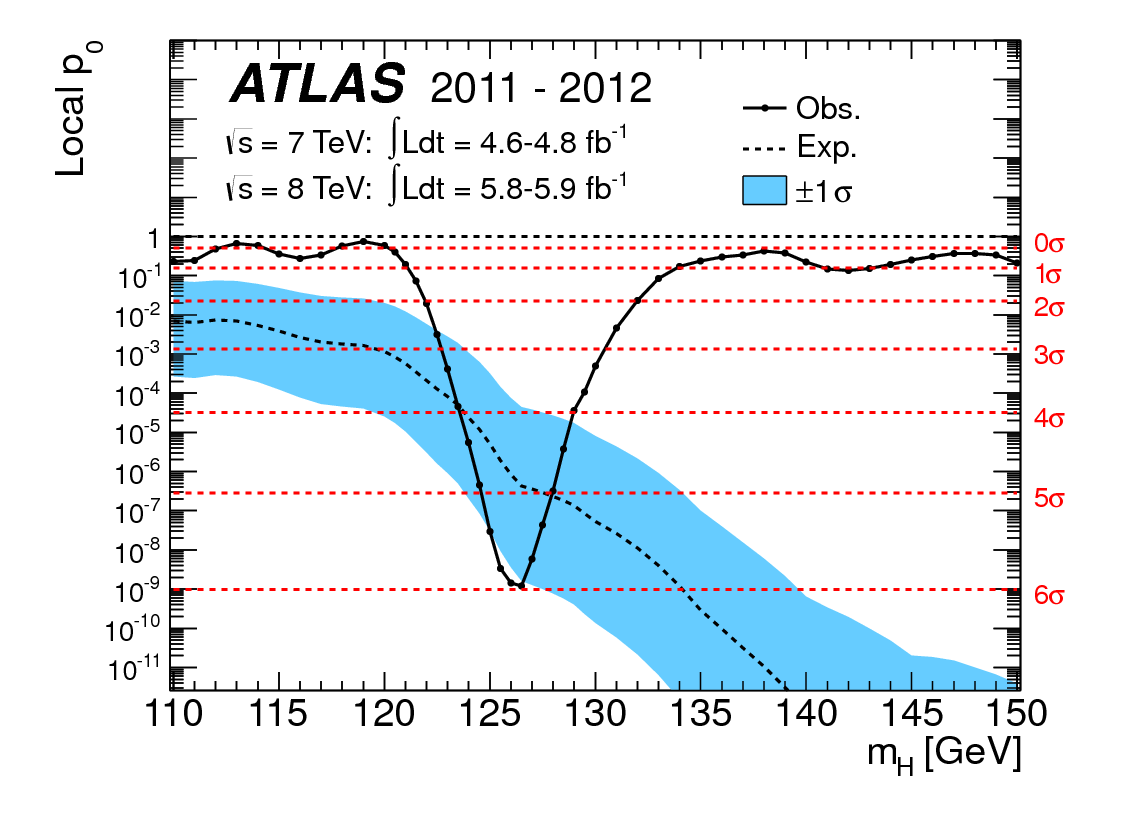
\includegraphics[keepaspectratio,alt={График p-value результата ATLAS}]{chapters/../assets/figures/Atlas_pvalue.png}}

}

\caption{Локальная статистическая значимость в результате ATLAS}

\end{figure}%

\begin{figure}[H]

{\centering \pandocbounded{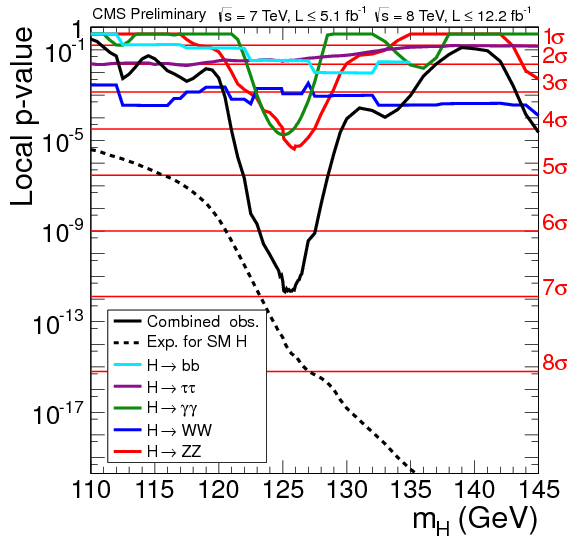
\includegraphics[keepaspectratio,alt={График p-value результата CMS}]{chapters/../assets/figures/CMS_pvalue.png}}

}

\caption{Локальная статистическая значимость в результате CMS}

\end{figure}%

За такими графиками стоят фоновая гипотеза, статистика теста,
\(p\)-value, преобразование вероятности в число стандартных отклонений и
учёт области поиска.

\subsection{Измерение и исключение в Daya
Bay}\label{ux438ux437ux43cux435ux440ux435ux43dux438ux435-ux438-ux438ux441ux43aux43bux44eux447ux435ux43dux438ux435-ux432-daya-bay}

Один эксперимент может как измерять параметр, так и исключать область
возможных значений.

\begin{figure}[H]

{\centering \pandocbounded{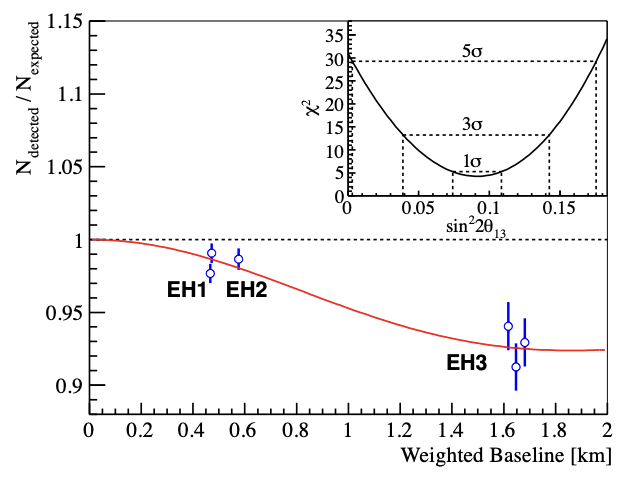
\includegraphics[keepaspectratio,alt={Измерение theta13 в Daya Bay}]{chapters/../assets/figures/DayaBayTheta13.png}}

}

\caption{Измерение ненулевого угла смешивания \(\theta_{13}\)}

\end{figure}%

\begin{figure}[H]

{\centering \pandocbounded{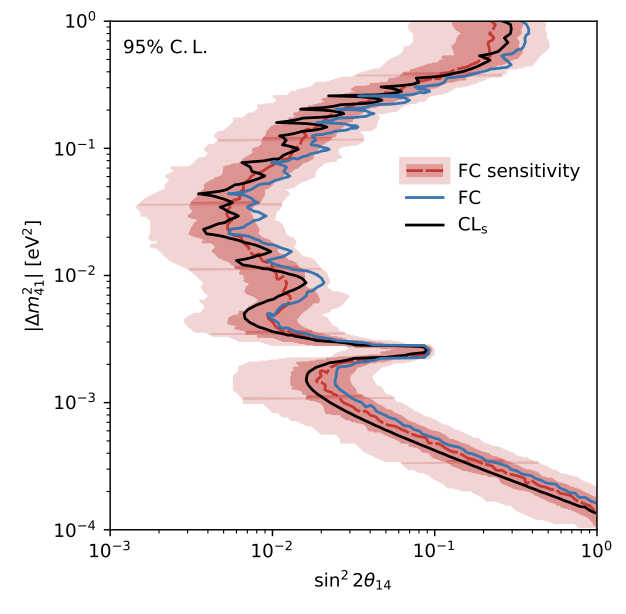
\includegraphics[keepaspectratio,alt={Исключение стерильных нейтрино в Daya Bay}]{chapters/../assets/figures/DBSterile.png}}

}

\caption{Исключение области параметров стерильных нейтрино}

\end{figure}%

В первом случае нужен best fit и неопределённость измерения. Во втором
--- процедура построения границы исключения. В обоих случаях одного
визуального сравнения кривых с точками недостаточно.

\section{Что скрыто в
графиках}\label{ux447ux442ux43e-ux441ux43aux440ux44bux442ux43e-ux432-ux433ux440ux430ux444ux438ux43aux430ux445}

Практически любой законченный физический результат опирается на один и
тот же набор идей:

\begin{itemize}
\tightlist
\item
  случайные флуктуации и распределения вероятности;
\item
  функция правдоподобия или \(\chi^2\);
\item
  оценка параметров и best fit;
\item
  доверительные интервалы и контуры;
\item
  статистическая значимость и \(p\)-value;
\item
  систематические неопределённости и корреляции;
\item
  nuisance-параметры и профилирование;
\item
  верхние пределы и области исключения.
\end{itemize}

Далее эти понятия будут вводиться по одному. Но уже сейчас полезно
увидеть весь процесс на простейшем примере.

\section{Первый фит: ширина
гауссианы}\label{ux43fux435ux440ux432ux44bux439-ux444ux438ux442-ux448ux438ux440ux438ux43dux430-ux433ux430ux443ux441ux441ux438ux430ux43dux44b}

Предположим, что экспериментальные события описываются гауссовым
распределением с известным центром \(x_0=0\) и неизвестной шириной
\(\sigma\):

\[
f(x;\sigma)
=
\frac{1}{\sqrt{2\pi}\sigma}
\exp\!\left(-\frac{x^2}{2\sigma^2}\right).
\]

Сгенерируем псевдоданные при некотором скрытом значении
\(\sigma_{\rm true}\). Затем переберём пробные значения \(\sigma\) и
сравним ожидаемое число событий \(\mu_i(\sigma)\) с наблюдаемым \(n_i\)
в каждом интервале.

Для сравнения используем пуассоновский deviance:

\[
\chi^2(\sigma)
=
2\sum_i
\left[
\mu_i(\sigma)-n_i
+n_i\ln\frac{n_i}{\mu_i(\sigma)}
\right],
\]

где для пустого интервала вклад с логарифмом принимается равным нулю.
Значение \(\widehat{\sigma}\), минимизирующее \(\chi^2(\sigma)\),
является best fit.

\subsection{Интерактив: найдите ширину
распределения}\label{ux438ux43dux442ux435ux440ux430ux43aux442ux438ux432-ux43dux430ux439ux434ux438ux442ux435-ux448ux438ux440ux438ux43dux443-ux440ux430ux441ux43fux440ux435ux434ux435ux43bux435ux43dux438ux44f}

Сначала меняйте только пробное значение \(\sigma\) и постарайтесь
визуально совместить модель с данными. Затем включите лучший фит и
истинное значение.

\begin{Shaded}
\begin{Highlighting}[]
\NormalTok{//| echo: false}

\NormalTok{viewof trialSigma = Inputs.range([0.35, 1.8], \{}
\NormalTok{  value: 0.75,}
\NormalTok{  step: 0.01,}
\NormalTok{  label: "Пробное значение σ"}
\NormalTok{\})}

\NormalTok{viewof nEvents = Inputs.range([250, 4000], \{}
\NormalTok{  value: 1200,}
\NormalTok{  step: 250,}
\NormalTok{  label: "Число событий"}
\NormalTok{\})}

\NormalTok{viewof regenerate = Inputs.button("Новые псевдоданные")}

\NormalTok{viewof showBest = Inputs.toggle(\{label: "Показать лучший фит", value: false\})}
\NormalTok{viewof showTruth = Inputs.toggle(\{label: "Показать истинное σ", value: false\})}

\NormalTok{function randnBook() \{}
\NormalTok{  const u = 1 {-} Math.random();}
\NormalTok{  const v = Math.random();}
\NormalTok{  return Math.sqrt({-}2 * Math.log(u)) * Math.cos(2 * Math.PI * v);}
\NormalTok{\}}

\NormalTok{centers = Array.from(\{length: 25\}, (\_, i) =\textgreater{} {-}3 + 0.25 * i)}
\NormalTok{dxBook = 0.25}
\NormalTok{xMinBook = centers[0] {-} dxBook / 2}
\NormalTok{xMaxBook = centers[centers.length {-} 1] + dxBook / 2}
\NormalTok{edgesBook = Array.from(\{length: centers.length + 1\}, (\_, i) =\textgreater{} xMinBook + i * dxBook)}
\NormalTok{curveXBook = Array.from(\{length: 401\}, (\_, i) =\textgreater{} xMinBook + (xMaxBook {-} xMinBook) * i / 400)}

\NormalTok{sigmaTrueBook = \{}
\NormalTok{  regenerate;}
\NormalTok{  return 0.55 + 0.75 * Math.random();}
\NormalTok{\}}

\NormalTok{function generateGaussianCountsBook(sigma, total) \{}
\NormalTok{  const counts = Array(centers.length).fill(0);}
\NormalTok{  let accepted = 0;}
\NormalTok{  while (accepted \textless{} total) \{}
\NormalTok{    const value = sigma * randnBook();}
\NormalTok{    if (value \textless{} xMinBook || value \textgreater{}= xMaxBook) continue;}
\NormalTok{    const index = Math.floor((value {-} xMinBook) / dxBook);}
\NormalTok{    counts[Math.max(0, Math.min(centers.length {-} 1, index))] += 1;}
\NormalTok{    accepted += 1;}
\NormalTok{  \}}
\NormalTok{  return counts;}
\NormalTok{\}}

\NormalTok{countsBook = \{}
\NormalTok{  regenerate;}
\NormalTok{  nEvents;}
\NormalTok{  return generateGaussianCountsBook(sigmaTrueBook, nEvents);}
\NormalTok{\}}

\NormalTok{totalBook = countsBook.reduce((sum, value) =\textgreater{} sum + value, 0)}

\NormalTok{function erfBook(x) \{}
\NormalTok{  const sign = x \textless{} 0 ? {-}1 : 1;}
\NormalTok{  const z = Math.abs(x);}
\NormalTok{  const t = 1 / (1 + 0.3275911 * z);}
\NormalTok{  const poly = (((((1.061405429 * t {-} 1.453152027) * t + 1.421413741) * t {-} 0.284496736) * t + 0.254829592) * t);}
\NormalTok{  return sign * (1 {-} poly * Math.exp({-}z * z));}
\NormalTok{\}}

\NormalTok{normalCdfBook = (x, sigma) =\textgreater{} 0.5 * (1 + erfBook(x / (Math.SQRT2 * sigma)))}

\NormalTok{function expectedCountsBook(sigma) \{}
\NormalTok{  const raw = centers.map((\_, i) =\textgreater{}}
\NormalTok{    normalCdfBook(edgesBook[i + 1], sigma) {-} normalCdfBook(edgesBook[i], sigma)}
\NormalTok{  );}
\NormalTok{  const norm = raw.reduce((sum, value) =\textgreater{} sum + value, 0);}
\NormalTok{  return raw.map((value) =\textgreater{} totalBook * value / norm);}
\NormalTok{\}}

\NormalTok{function devianceBook(sigma) \{}
\NormalTok{  const expected = expectedCountsBook(sigma);}
\NormalTok{  return countsBook.reduce((sum, observed, i) =\textgreater{} \{}
\NormalTok{    const mean = Math.max(expected[i], 1e{-}12);}
\NormalTok{    return observed \textgreater{} 0}
\NormalTok{      ? sum + 2 * (mean {-} observed + observed * Math.log(observed / mean))}
\NormalTok{      : sum + 2 * mean;}
\NormalTok{  \}, 0);}
\NormalTok{\}}

\NormalTok{sigmaGridBook = Array.from(\{length: 291\}, (\_, i) =\textgreater{} 0.35 + 0.005 * i)}
\NormalTok{profileBook = sigmaGridBook.map((sigma) =\textgreater{} (\{sigma, chi2: devianceBook(sigma)\}))}
\NormalTok{bestBook = profileBook.reduce((a, b) =\textgreater{} a.chi2 \textless{} b.chi2 ? a : b)}
\NormalTok{trialChi2Book = devianceBook(trialSigma)}

\NormalTok{function smoothCurveBook(sigma) \{}
\NormalTok{  const truncation = normalCdfBook(xMaxBook, sigma) {-} normalCdfBook(xMinBook, sigma);}
\NormalTok{  const scale = totalBook * dxBook / (Math.sqrt(2 * Math.PI) * sigma * truncation);}
\NormalTok{  return curveXBook.map((x) =\textgreater{} (\{}
\NormalTok{    x,}
\NormalTok{    y: scale * Math.exp({-}(x * x) / (2 * sigma * sigma))}
\NormalTok{  \}));}
\NormalTok{\}}

\NormalTok{fitPlotBook = Plot.plot(\{}
\NormalTok{  width: 760,}
\NormalTok{  height: 410,}
\NormalTok{  marginLeft: 58,}
\NormalTok{  x: \{label: "x", grid: true\},}
\NormalTok{  y: \{label: "число событий", grid: true\},}
\NormalTok{  marks: [}
\NormalTok{    Plot.rectY(centers.map((x, i) =\textgreater{} (\{x, y: countsBook[i]\})), \{}
\NormalTok{      x1: (d) =\textgreater{} d.x {-} dxBook / 2,}
\NormalTok{      x2: (d) =\textgreater{} d.x + dxBook / 2,}
\NormalTok{      y: "y",}
\NormalTok{      fill: "\#dce8ee",}
\NormalTok{      stroke: "\#486979"}
\NormalTok{    \}),}
\NormalTok{    Plot.line(smoothCurveBook(trialSigma), \{}
\NormalTok{      x: "x", y: "y", stroke: "\#c7472f", strokeWidth: 3}
\NormalTok{    \}),}
\NormalTok{    ...(showBest ? [Plot.line(smoothCurveBook(bestBook.sigma), \{}
\NormalTok{      x: "x", y: "y", stroke: "\#147d64", strokeWidth: 3, strokeDasharray: "7,5"}
\NormalTok{    \})] : []),}
\NormalTok{    ...(showTruth ? [Plot.line(smoothCurveBook(sigmaTrueBook), \{}
\NormalTok{      x: "x", y: "y", stroke: "\#2a5ea8", strokeWidth: 2.5}
\NormalTok{    \})] : [])}
\NormalTok{  ]}
\NormalTok{\})}

\NormalTok{profilePlotBook = Plot.plot(\{}
\NormalTok{  width: 560,}
\NormalTok{  height: 410,}
\NormalTok{  marginLeft: 58,}
\NormalTok{  x: \{label: "σ", grid: true\},}
\NormalTok{  y: \{label: "χ²(σ)", grid: true\},}
\NormalTok{  marks: [}
\NormalTok{    Plot.line(profileBook, \{x: "sigma", y: "chi2", stroke: "\#486979", strokeWidth: 2.5\}),}
\NormalTok{    Plot.dot([\{sigma: trialSigma, chi2: trialChi2Book\}], \{}
\NormalTok{      x: "sigma", y: "chi2", fill: "\#c7472f", r: 6}
\NormalTok{    \}),}
\NormalTok{    ...(showBest ? [Plot.dot([bestBook], \{}
\NormalTok{      x: "sigma", y: "chi2", fill: "\#147d64", r: 6}
\NormalTok{    \})] : [])}
\NormalTok{  ]}
\NormalTok{\})}

\NormalTok{html\textasciigrave{}}
\NormalTok{\textless{}div class="book{-}fit{-}output"\textgreater{}}
\NormalTok{  \textless{}div class="book{-}fit{-}plots"\textgreater{}}
\NormalTok{    \textless{}figure\textgreater{}$\{fitPlotBook\}\textless{}figcaption\textgreater{}Псевдоданные и пробная модель\textless{}/figcaption\textgreater{}\textless{}/figure\textgreater{}}
\NormalTok{    \textless{}figure\textgreater{}$\{profilePlotBook\}\textless{}figcaption\textgreater{}Профиль функции χ²\textless{}/figcaption\textgreater{}\textless{}/figure\textgreater{}}
\NormalTok{  \textless{}/div\textgreater{}}
\NormalTok{  \textless{}div class="book{-}fit{-}readout"\textgreater{}}
\NormalTok{    \textless{}span\textgreater{}\textless{}b\textgreater{}Ваш выбор\textless{}/b\textgreater{} σ = $\{trialSigma.toFixed(2)\}, χ² = $\{trialChi2Book.toFixed(1)\}\textless{}/span\textgreater{}}
\NormalTok{    $\{showBest ? \textasciigrave{}\textless{}span class="fit{-}best"\textgreater{}\textless{}b\textgreater{}Best fit\textless{}/b\textgreater{} σ̂ = $\{bestBook.sigma.toFixed(3)\}\textless{}/span\textgreater{}\textasciigrave{} : \textasciigrave{}\textasciigrave{}\}}
\NormalTok{    $\{showTruth ? \textasciigrave{}\textless{}span class="fit{-}truth"\textgreater{}\textless{}b\textgreater{}Истина\textless{}/b\textgreater{} σ = $\{sigmaTrueBook.toFixed(3)\}\textless{}/span\textgreater{}\textasciigrave{} : \textasciigrave{}\textasciigrave{}\}}
\NormalTok{  \textless{}/div\textgreater{}}
\NormalTok{\textless{}/div\textgreater{}}
\NormalTok{\textasciigrave{}}
\end{Highlighting}
\end{Shaded}

Интерактив показывает несколько общих принципов.

\begin{enumerate}
\def\labelenumi{\arabic{enumi}.}
\tightlist
\item
  Одни и те же данные допускают множество моделей, но согласуются с ними
  по-разному.
\item
  Визуальное совпадение полезно, однако численный критерий делает
  сравнение воспроизводимым.
\item
  Best fit не обязан совпадать с истинным параметром: оценка флуктуирует
  вместе с данными.
\item
  При увеличении числа событий профиль становится уже --- данные точнее
  ограничивают \(\sigma\).
\end{enumerate}

\section{Итоги
главы}\label{ux438ux442ux43eux433ux438-ux433ux43bux430ux432ux44b}

\begin{itemize}
\tightlist
\item
  Статистическая модель связывает теоретическое предсказание и
  наблюдаемые данные.
\item
  Физический результат всегда зависит не только от данных, но и от
  выбранной процедуры анализа.
\item
  Частотный и байесовский подходы по-разному интерпретируют вероятность.
\item
  Параметр \(\theta\) и его оценка \(\widehat{\theta}\) --- разные
  объекты.
\item
  Даже простейший фит уже содержит данные, модель, функцию сравнения и
  процедуру оценки параметра.
\end{itemize}

\section{Что
дальше}\label{ux447ux442ux43e-ux434ux430ux43bux44cux448ux435}

Следующая глава вводит случайные величины, математическое ожидание и
моменты --- основные строительные блоки вероятностных моделей.

\href{01_random_distributions.qmd}{Перейти к главе «Случайные величины,
распределения, моменты»}

\chapter{Случайные величины, распределения,
моменты}\label{ux441ux43bux443ux447ux430ux439ux43dux44bux435-ux432ux435ux43bux438ux447ux438ux43dux44b-ux440ux430ux441ux43fux440ux435ux434ux435ux43bux435ux43dux438ux44f-ux43cux43eux43cux435ux43dux442ux44b}

Главная мысль

Флуктуации данных в эксперименте носят вероятностный характер. В
зависимости от физики задачи подбирается подходящее распределение.

\section{План
главы}\label{ux43fux43bux430ux43d-ux433ux43bux430ux432ux44b}

\begin{itemize}
\tightlist
\item
  Случайность и случайные величины
\item
  Средние, дисперсии и моменты
\item
  Базовые распределения
\item
  Счёт успехов: биномиальная модель
\item
  Счёт редких событий: пуассоновская модель
\item
  Непрерывные ошибки: нормальная модель
\item
  Резюме
\end{itemize}

\section{Случайность и случайные
величины}\label{ux441ux43bux443ux447ux430ux439ux43dux43eux441ux442ux44c-ux438-ux441ux43bux443ux447ux430ux439ux43dux44bux435-ux432ux435ux43bux438ux447ux438ux43dux44b}

{\def\LTcaptype{none} % do not increment counter
\begin{longtable}[]{@{}
  >{\centering\arraybackslash}p{(\linewidth - 4\tabcolsep) * \real{0.4909}}
  >{\centering\arraybackslash}p{(\linewidth - 4\tabcolsep) * \real{0.1636}}
  >{\centering\arraybackslash}p{(\linewidth - 4\tabcolsep) * \real{0.3364}}@{}}
\toprule\noalign{}
\endhead
\bottomrule\noalign{}
\endlastfoot
& \textbf{Случайность} & \\
\textbf{\emph{Классическая физика}} & & \textbf{\emph{Квантовая
физика}} \\
Случайность возникает из-за неполного знания

начальных условий и большого числа степеней свободы & & Случайность
заложена в саму теорию \\
\end{longtable}
}

Эксперимент наблюдает не «идеальное ожидание» , а конкретную реализацию
со статическими флуктуациями. Поэтому сравнение модели с данными всегда
формулируется на языке вероятности.

\begin{description}
\item[\textbf{Случайная величина} \(X:\)]
Экспериментально измеряемая величина, которая не может быть предсказана
до проведения эксперимента.
\end{description}

\textbf{Дискретная} \(X\) описывается \textbf{\emph{функцией вероятности
(PMF -- probability mass function):}}

\[p_k=P(X=x_k), \quad \sum_k p_k=1.\]

\textbf{Непрерывная} \(X\) --- \textbf{\emph{плотностью вероятности}}
\textbf{\emph{(PDF -- probability density function):}}

\[P(x\leq X<x+dx)=f(x)dx, \quad \int_{-\infty}^{+\infty}f(x)dx=1.\]

В обеих записях последние выражения являются соответсвующими условиями
нормировки.

\subsection{Кумулятивная функция распределения
(CDF)}\label{ux43aux443ux43cux443ux43bux44fux442ux438ux432ux43dux430ux44f-ux444ux443ux43dux43aux446ux438ux44f-ux440ux430ux441ux43fux440ux435ux434ux435ux43bux435ux43dux438ux44f-cdf}

Для непрерывной \(X\):

\[F(a)=P(X<a)=\int_{-\infty}^a f(x)dx.\]

С математической точки зрения, CDF отражает вероятность того, что
\(X<a.\) \(F(a)\) монотонно возрастает от 0 до 1 при изменении
\(a \in (-\infty,\infty)\). Заметим, что для непрерывных распределений
справедливо следующее свойство:

\[F'(a)=f(a).\]

При помощи кумулятивной функции распределения легко вычислить
\textbf{\emph{вероятность попасть в интервал}} \([a,b):\)

\[P(a\leq X<b)=F(b)-F(a).\]

\section{Средние, дисперсии и
моменты}\label{ux441ux440ux435ux434ux43dux438ux435-ux434ux438ux441ux43fux435ux440ux441ux438ux438-ux438-ux43cux43eux43cux435ux43dux442ux44b}

\subsection{Моменты
распределения}\label{ux43cux43eux43cux435ux43dux442ux44b-ux440ux430ux441ux43fux440ux435ux434ux435ux43bux435ux43dux438ux44f}

\begin{description}
\item[\textbf{\emph{Момент функции}}:]
\[\langle x^n\rangle=\mathbb{E}[X^n]=\int_{-\infty}^\infty x^nf(x)dx.\]
\end{description}

Если известны все моменты \(\langle x^n\rangle\), то можно восстановить
\(f(x)\), но это распространяется не на все функции.

\subsection{Практически важные
моменты}\label{ux43fux440ux430ux43aux442ux438ux447ux435ux441ux43aux438-ux432ux430ux436ux43dux44bux435-ux43cux43eux43cux435ux43dux442ux44b}

{\def\LTcaptype{none} % do not increment counter
\begin{longtable}[]{@{}
  >{\centering\arraybackslash}p{(\linewidth - 2\tabcolsep) * \real{0.1465}}
  >{\centering\arraybackslash}p{(\linewidth - 2\tabcolsep) * \real{0.8535}}@{}}
\toprule\noalign{}
\begin{minipage}[b]{\linewidth}\centering
Момент
\end{minipage} & \begin{minipage}[b]{\linewidth}\centering
Формула
\end{minipage} \\
\midrule\noalign{}
\endhead
\bottomrule\noalign{}
\endlastfoot
Среднее &
\(\mu=\langle x\rangle=\mathbb{E}[X]=\int_{-\infty}^{+\infty} xf(x)dx\) \\
Средний квадрат &
\(\langle x^2\rangle=\mathbb{E}[X^2]=\int_{-\infty}^{+\infty} x^2 f(x)dx\) \\
Дисперсия (вариация) &
\(\sigma^2=Var(X)=\mathbb{E}\left[(X-\mu)^2\right]=\mathbb{E}\left[X^2-2\mu X+\mu^2\right]=\langle x^2 \rangle-\langle x\rangle^2\) \\
\end{longtable}
}

\subsection{\texorpdfstring{Моменты распределения произвольной функции
\(g(X)\) случайной
величины}{Моменты распределения произвольной функции g(X) случайной величины}}\label{ux43cux43eux43cux435ux43dux442ux44b-ux440ux430ux441ux43fux440ux435ux434ux435ux43bux435ux43dux438ux44f-ux43fux440ux43eux438ux437ux432ux43eux43bux44cux43dux43eux439-ux444ux443ux43dux43aux446ux438ux438-gx-ux441ux43bux443ux447ux430ux439ux43dux43eux439-ux432ux435ux43bux438ux447ux438ux43dux44b}

{\def\LTcaptype{none} % do not increment counter
\begin{longtable}[]{@{}
  >{\centering\arraybackslash}p{(\linewidth - 2\tabcolsep) * \real{0.1965}}
  >{\centering\arraybackslash}p{(\linewidth - 2\tabcolsep) * \real{0.8035}}@{}}
\toprule\noalign{}
\begin{minipage}[b]{\linewidth}\centering
Момент
\end{minipage} & \begin{minipage}[b]{\linewidth}\centering
Формула
\end{minipage} \\
\midrule\noalign{}
\endhead
\bottomrule\noalign{}
\endlastfoot
Среднее значение функции \(g(X)\) &
\(\langle g(x)\rangle=\mathbb{E}\left[g(X)\right]=\int_{-\infty}^{+\infty} g(x)f(x)dx\) \\
Вариация функции \(g(X)\) &
\(Var(g(X))=\mathbb{E}\left[(g(X)-\langle g(X)\rangle)^2\right]= \int_{-\infty}^\infty \left(g(x)-\langle g(x)\rangle\right)^2 f(x) dx\) \\
\end{longtable}
}

\section{Базовые
распределения}\label{ux431ux430ux437ux43eux432ux44bux435-ux440ux430ux441ux43fux440ux435ux434ux435ux43bux435ux43dux438ux44f}

В рамках данной главы мы рассмотрим три важных примера:

\begin{itemize}
\item
  Биномиальное распределение
\item
  Распределение Пуассона
\item
  Нормальное (гауссово) распределение
\end{itemize}

\section{Счёт успехов: биномиальная
модель}\label{ux441ux447ux451ux442-ux443ux441ux43fux435ux445ux43eux432-ux431ux438ux43dux43eux43cux438ux430ux43bux44cux43dux430ux44f-ux43cux43eux434ux435ux43bux44c}

Если в \(n\) независимых испытаниях вероятность успеха равна \(p\), то

\[P(K=k)=\begin{pmatrix} n\\k\end{pmatrix}p^k(1-p)^{n-k}, \quad k=0,\dots,n,\]

где

\[\begin{pmatrix} n\\k\end{pmatrix}=\frac{n!}{k!(n-k)!}\]

это число способов выбрать \(k\) успехов среди \(n\) испытаний.

\subsection{Пример биномиального
распределения}\label{ux43fux440ux438ux43cux435ux440-ux431ux438ux43dux43eux43cux438ux430ux43bux44cux43dux43eux433ux43e-ux440ux430ux441ux43fux440ux435ux434ux435ux43bux435ux43dux438ux44f}

Пронаблюдаем \(n\) распадов \(W^{\pm}\). Число распадов \(W\to\mu\nu\):

\[k\sim\mathrm{Bin}(n,p),\]

где \(p\) --- вероятность такого распада. Построим на одних осях три
случая: \(n=5,20,100\) при \(p=0.3\).

\begin{Shaded}
\begin{Highlighting}[]
\ImportTok{from}\NormalTok{ math }\ImportTok{import}\NormalTok{ comb}
\ImportTok{import}\NormalTok{ numpy }\ImportTok{as}\NormalTok{ np}

\NormalTok{p }\OperatorTok{=} \FloatTok{0.3}
\ControlFlowTok{for}\NormalTok{ n }\KeywordTok{in}\NormalTok{ [}\DecValTok{5}\NormalTok{, }\DecValTok{20}\NormalTok{, }\DecValTok{100}\NormalTok{]:}
\NormalTok{    k }\OperatorTok{=}\NormalTok{ np.arange(n }\OperatorTok{+} \DecValTok{1}\NormalTok{)}
\NormalTok{    pmf }\OperatorTok{=}\NormalTok{ np.array([comb(n, i) }\OperatorTok{*}\NormalTok{ p}\OperatorTok{**}\NormalTok{i }\OperatorTok{*}\NormalTok{ (}\DecValTok{1}\OperatorTok{{-}}\NormalTok{p)}\OperatorTok{**}\NormalTok{(n}\OperatorTok{{-}}\NormalTok{i) }\ControlFlowTok{for}\NormalTok{ i }\KeywordTok{in}\NormalTok{ k])}
\end{Highlighting}
\end{Shaded}

\begin{figure}[H]

{\centering \pandocbounded{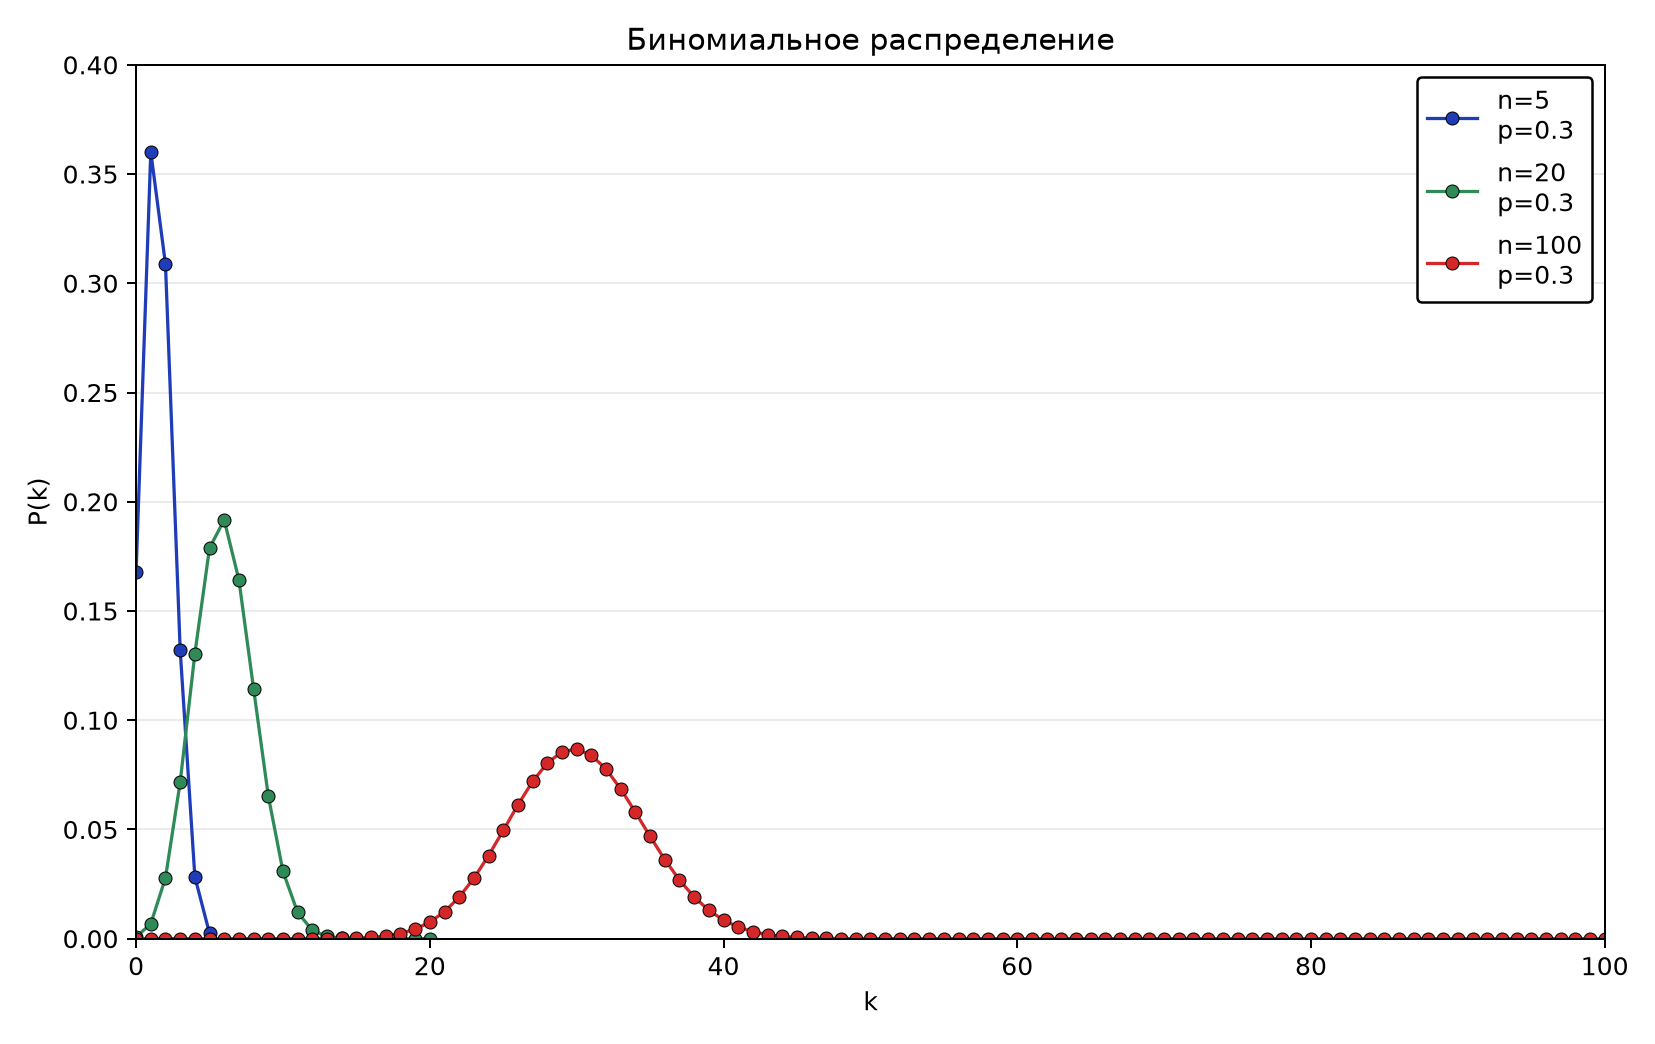
\includegraphics[keepaspectratio]{chapters/../assets/figures/binomial_pmf_profiles.png}}

}

\caption{Примеры биномиального распределения}

\end{figure}%

Обратите внимание, что с увеличением \(n\) биномиальное распределение
переходит в распределение Гаусса (красная кривая).

\subsection{Моменты биномиального
распределения}\label{ux43cux43eux43cux435ux43dux442ux44b-ux431ux438ux43dux43eux43cux438ux430ux43bux44cux43dux43eux433ux43e-ux440ux430ux441ux43fux440ux435ux434ux435ux43bux435ux43dux438ux44f}

\begin{itemize}
\item
  \textbf{Математическое ожидание:} \(\mathbb{E}[K]=np\)
\item
  \textbf{Дисперсия:} \(Var(K)=np(1-p)\)
\item
  \textbf{Пример:} число распадов нужного канала при фиксированном числе
  родительских частиц
\end{itemize}

\subsubsection{\texorpdfstring{\textbf{Вывод}
\(\mathbb{E}[K]\)}{Вывод \textbackslash mathbb\{E\}{[}K{]}}}\label{ux432ux44bux432ux43eux434-mathbbek}

По определению:

\[\mathbb{E}[K]=\sum_{k=0}^n kP(K=k)=\sum_{k=0}^n k \begin{pmatrix} n\\k\end{pmatrix} p^k(1-p)^{n-k}.\]

Используя тождество:

\[k \begin{pmatrix} n\\k\end{pmatrix}=k\frac{n!}{k!(n-k)!}=n\frac{(n-1)!}{(k-1)!(n-k)!}=n\begin{pmatrix} n-1\\k-1\end{pmatrix},\]

получим

\[\mathbb{E}[K]=np\sum_{k=1}^n \begin{pmatrix} n-1\\k-1\end{pmatrix}p^{k-1}(1-p)^{n-k}.\]

Положим \(j=k-1\):

\[\mathbb{E}[K]=np\sum_{j=0}^{n-1} \begin{pmatrix} n-1\\j\end{pmatrix}p^{j}(1-p)^{(n-1)-j},\]

тогда по биному Ньютона:

\[\sum_{j=0}^{n-1} \begin{pmatrix} n-1\\j\end{pmatrix}p^{j}(1-p)^{(n-1)-j}=(p+(1-p))^{n-1}=1.\]

Итог:

\[\mathbb{E}[K]=np. \quad \blacksquare\]

\subsubsection{\texorpdfstring{\textbf{Вывод}
\(Var(K)\)}{Вывод Var(K)}}\label{ux432ux44bux432ux43eux434-vark}

Начнем со второго факториального момента:

\[\mathbb{E}[K(K-1)]=\sum_{k=0}^n k(k-1) \begin{pmatrix} n\\k\end{pmatrix} p^k(1-p)^{n-k}.\]

Используя тождество:

\[k(k-1) \begin{pmatrix} n\\k\end{pmatrix}=k(k-1)\frac{n!}{k!(n-k)!}=n(n-1)\frac{(n-2)!}{(k-2)!(n-k)!}=n(n-1)\begin{pmatrix} n-2\\k-2\end{pmatrix},\]

получим

\[\mathbb{E}[K(K-1)]=n(n-1)p^2\sum_{k=2}^n \begin{pmatrix} n-2\\k-2\end{pmatrix} p^{k-2}(1-p)^{n-k}=n(n-1)p^2.\]

Воспользуемся разложением \(K^2\):

\[K^2=K(K-1)+K,\]

тогда

\[\mathbb{E}[K^2]=\mathbb{E}[K(K-1)]+\mathbb{E}[K]=n(n-1)p^2+np.\]

Таким образом, вариацию \(Var(K)\) можно записать в виде:

\[Var(K)=\mathbb{E}[K^2]-\mathbb{E}[K]^2=\left(n(n-1)p^2+np\right)-(np)^2.\]

Итог:

\[Var(K)=np(1-p). \quad \blacksquare\]

\section{Счёт редких событий: пуассоновская
модель}\label{ux441ux447ux451ux442-ux440ux435ux434ux43aux438ux445-ux441ux43eux431ux44bux442ux438ux439-ux43fux443ux430ux441ux441ux43eux43dux43eux432ux441ux43aux430ux44f-ux43cux43eux434ux435ux43bux44c}

\textbf{Распределение Пуассона} моделирует число событий в фиксированном
интервале времени или пространства при постоянной средней интенсивности
\(λ\) и независимых событиях.

Вероятность наблюдения~\(N=k\)~событий при среднем числе событий \(λ\):

\[P(N=k)=\frac{\lambda^k e^{-\lambda}}{k!}, \quad k=0,1,2,\dots\]

Пример: число распадов радиоактивного источника за 1 минуту.

\subsection{Пример распределения
Пуассона}\label{ux43fux440ux438ux43cux435ux440-ux440ux430ux441ux43fux440ux435ux434ux435ux43bux435ux43dux438ux44f-ux43fux443ux430ux441ux441ux43eux43dux430}

Посчитаем число событий \(N\) за фиксированное время. Если среднее число
событий равно \(\lambda\), то

\[N\sim \mathrm{Pois}(\lambda).\]

Построим на одних осях три случая: \(\lambda=1,4,10\).

\begin{Shaded}
\begin{Highlighting}[]
\ImportTok{from}\NormalTok{ math }\ImportTok{import}\NormalTok{ factorial}
\ImportTok{import}\NormalTok{ numpy }\ImportTok{as}\NormalTok{ np}

\ControlFlowTok{for}\NormalTok{ lam }\KeywordTok{in}\NormalTok{ [}\DecValTok{1}\NormalTok{, }\DecValTok{4}\NormalTok{, }\DecValTok{10}\NormalTok{]:}
\NormalTok{    k }\OperatorTok{=}\NormalTok{ np.arange(}\DecValTok{26}\NormalTok{)}
\NormalTok{    pmf }\OperatorTok{=}\NormalTok{ np.exp(}\OperatorTok{{-}}\NormalTok{lam) }\OperatorTok{*}\NormalTok{ lam}\OperatorTok{**}\NormalTok{k }\OperatorTok{/}\NormalTok{ np.array([factorial(i) }\ControlFlowTok{for}\NormalTok{ i }\KeywordTok{in}\NormalTok{ k])}
\end{Highlighting}
\end{Shaded}

\begin{figure}[H]

{\centering \pandocbounded{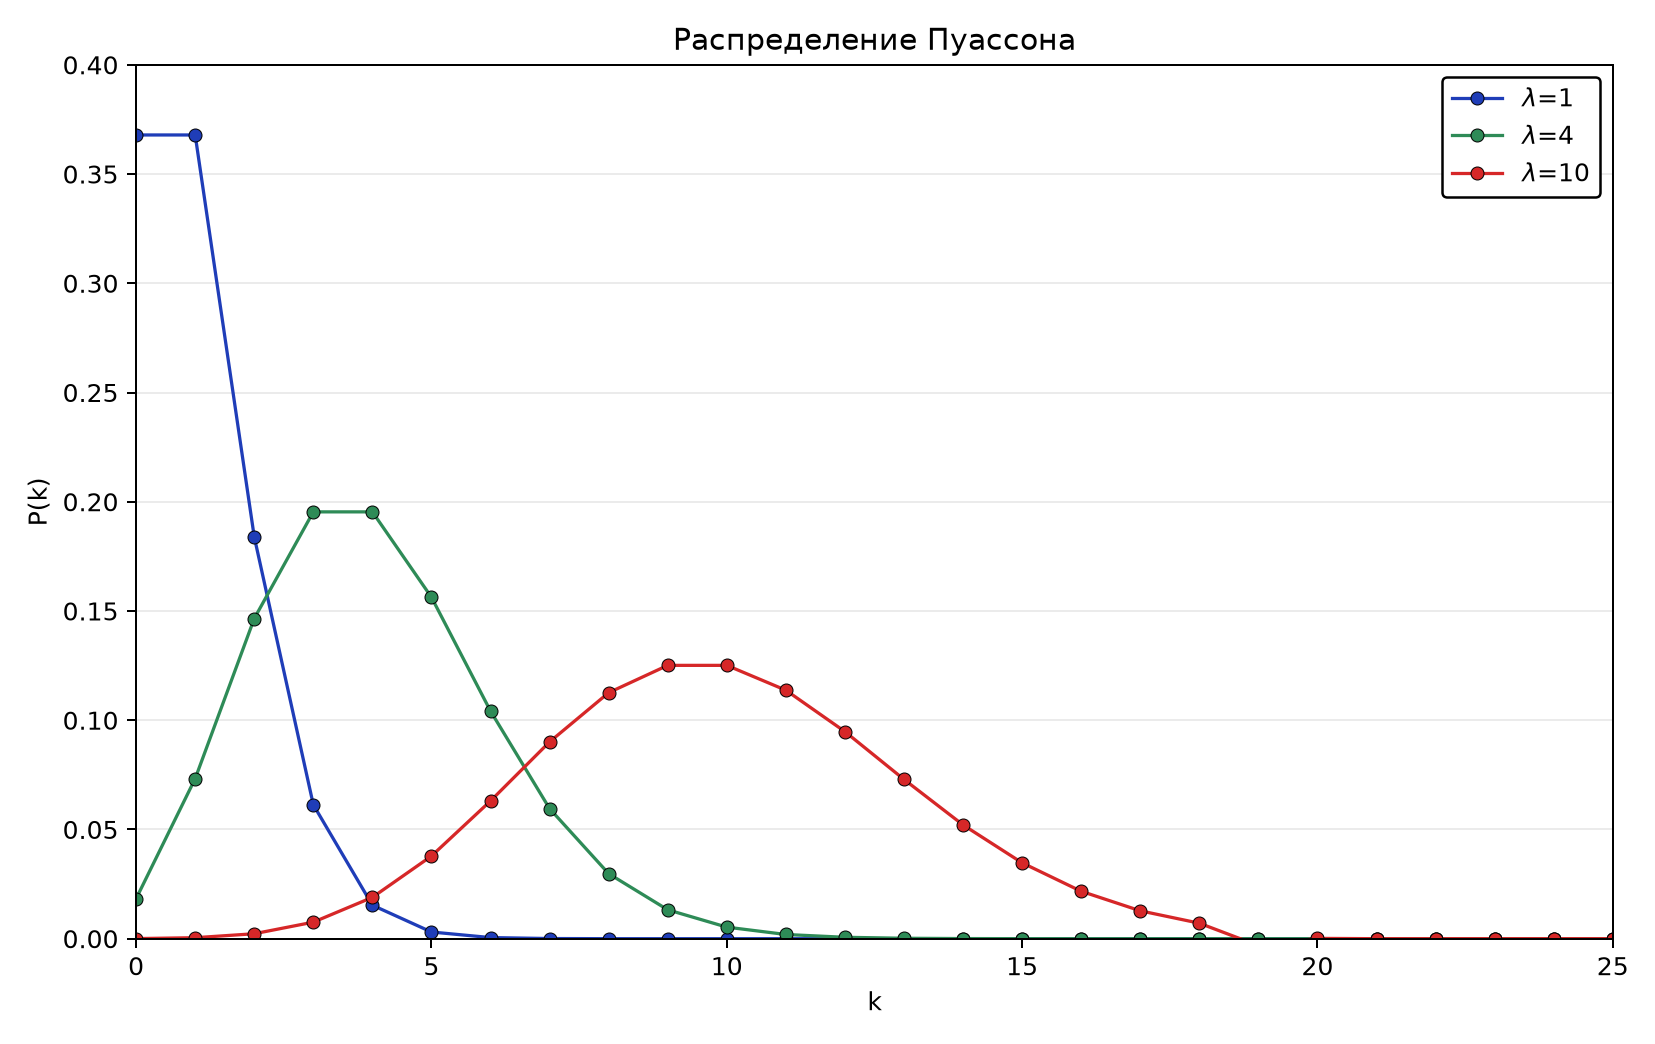
\includegraphics[keepaspectratio]{chapters/../assets/figures/poisson_pmf_profiles.png}}

}

\caption{Примеры распределения Пуассона}

\end{figure}%

Обратите внимание, что с увеличением \(n\) распределение Пуассона также
стремиться к нормальному распределению (красная кривая).

\subsection{Моменты распределения
Пуассона}\label{ux43cux43eux43cux435ux43dux442ux44b-ux440ux430ux441ux43fux440ux435ux434ux435ux43bux435ux43dux438ux44f-ux43fux443ux430ux441ux441ux43eux43dux430}

\begin{itemize}
\item
  \textbf{Математическое ожидание:} \(\mathbb{E}[K]=\lambda\)
\item
  \textbf{Дисперсия:} \(Var(K)=\lambda\)
\end{itemize}

\subsubsection{\texorpdfstring{\textbf{Вывод}
\(\mathbb{E}[N]\)}{Вывод \textbackslash mathbb\{E\}{[}N{]}}}\label{ux432ux44bux432ux43eux434-mathbben}

По определению:

\[\mathbb{E}[N]=\sum_{k=0}^\infty k\frac{\lambda^k e^{-\lambda}}{k!}.\]

Вынесем множитель за сумму:

\[\mathbb{E}[N]=\lambda e^{-\lambda}\sum_{k=1}^\infty \frac{\lambda^{k-1} }{(k-1)!}.\]

Сдвинем индекс \(j=k-1\), не забыв разложение экспоненты в ряд Тейлора :

\[\mathbb{E}[N]=\lambda e^{-\lambda}\sum_{j=0}^\infty \frac{\lambda^{j} }{j!}=\lambda e^{-\lambda}e^{\lambda}=\lambda.\]

Итог:

\[\mathbb{E}[N]=\lambda. \quad \blacksquare\]

\subsubsection{\texorpdfstring{\textbf{Вывод}
\(Var(N)\)}{Вывод Var(N)}}\label{ux432ux44bux432ux43eux434-varn}

Воспользуемся уже знакомым вторым факториальным моментом:

\[\mathbb{E}[N(N-1)]=\sum_{k=0}^\infty k(k-1)\frac{\lambda^k e^{-\lambda}}{k!}.\]

Поскольку

\[\frac{k(k-1)}{k!}=\frac{1}{(k-2)!},\]

то можно преобразовать выражение для момента:

\[\mathbb{E}[N(N-1)]=\lambda^2 e^{-\lambda}\sum_{k=2}^\infty \frac{\lambda^{k-2} }{(k-2)!}=\lambda^2 e^{-\lambda}\sum_{j=0}^\infty \frac{\lambda^{j} }{j!}=\lambda^2.\]

Используя связь:

\[N^2=N(N-1)+N,\]

получим

\[\mathbb{E}[N^2]=\mathbb{E}[N(N-1)]+\mathbb{E}[N]=\lambda^2+\lambda.\]

Таким образом, вариацию \(Var(N)\) можно записать в виде:

\[Var(N)=\mathbb{E}[N^2]-\mathbb{E}[N]^2=(\lambda^2+\lambda)-\lambda^2=\lambda.\]

Итог:

\[Var(N)=\lambda. \quad \blacksquare\]

\section{Непрерывные ошибки: нормальная
модель}\label{ux43dux435ux43fux440ux435ux440ux44bux432ux43dux44bux435-ux43eux448ux438ux431ux43aux438-ux43dux43eux440ux43cux430ux43bux44cux43dux430ux44f-ux43cux43eux434ux435ux43bux44c}

\subsection{Нормальное (гауссово)
распределение}\label{ux43dux43eux440ux43cux430ux43bux44cux43dux43eux435-ux433ux430ux443ux441ux441ux43eux432ux43e-ux440ux430ux441ux43fux440ux435ux434ux435ux43bux435ux43dux438ux435}

\[f(x;\mu,\sigma)=\frac{1}{\sigma (2\pi)^{1/2}}\exp\left[-\frac{(x-\mu)^2}{2\sigma^2}\right],\]

где \(\mu\) -- среднее значение, \(\sigma\) - дисперсия случайной
величины.

Оно часто представимо в виде суммы многих малых независимых вкладов.

Так почему же распределение «нормальное»?

\begin{quote}
Много лет назад я назвал кривую Лапласа-Гаусса нормальной кривой. Это
название, избегая международного спора о приоритете, имеет недостаток:
оно заставляет думать, что все прочие распределения частот в том или
ином смысле «ненормальны».

К. Пирсон (1920)
\end{quote}

\subsection{Пример нормального
распределения}\label{ux43fux440ux438ux43cux435ux440-ux43dux43eux440ux43cux430ux43bux44cux43dux43eux433ux43e-ux440ux430ux441ux43fux440ux435ux434ux435ux43bux435ux43dux438ux44f}

Параметр \(\mu\) задаёт среднее значение, \(\sigma\) --- ширину разброса
величины. Построим на одних осях три случая:
\((\mu,\sigma)=(0,1),(0,2),(2,1)\).

\begin{Shaded}
\begin{Highlighting}[]
\ImportTok{import}\NormalTok{ numpy }\ImportTok{as}\NormalTok{ np}

\NormalTok{x }\OperatorTok{=}\NormalTok{ np.linspace(}\OperatorTok{{-}}\DecValTok{6}\NormalTok{, }\DecValTok{6}\NormalTok{, }\DecValTok{400}\NormalTok{)}
\ControlFlowTok{for}\NormalTok{ mu, sigma }\KeywordTok{in}\NormalTok{ [(}\DecValTok{0}\NormalTok{, }\DecValTok{1}\NormalTok{), (}\DecValTok{0}\NormalTok{, }\DecValTok{2}\NormalTok{), (}\DecValTok{2}\NormalTok{, }\DecValTok{1}\NormalTok{)]:}
\NormalTok{    pdf }\OperatorTok{=}\NormalTok{ np.exp(}\OperatorTok{{-}}\FloatTok{0.5}\OperatorTok{*}\NormalTok{((x}\OperatorTok{{-}}\NormalTok{mu)}\OperatorTok{/}\NormalTok{sigma)}\OperatorTok{**}\DecValTok{2}\NormalTok{)}\OperatorTok{/}\NormalTok{(sigma}\OperatorTok{*}\NormalTok{np.sqrt(}\DecValTok{2}\OperatorTok{*}\NormalTok{np.pi))}
\end{Highlighting}
\end{Shaded}

\begin{figure}[H]

{\centering \pandocbounded{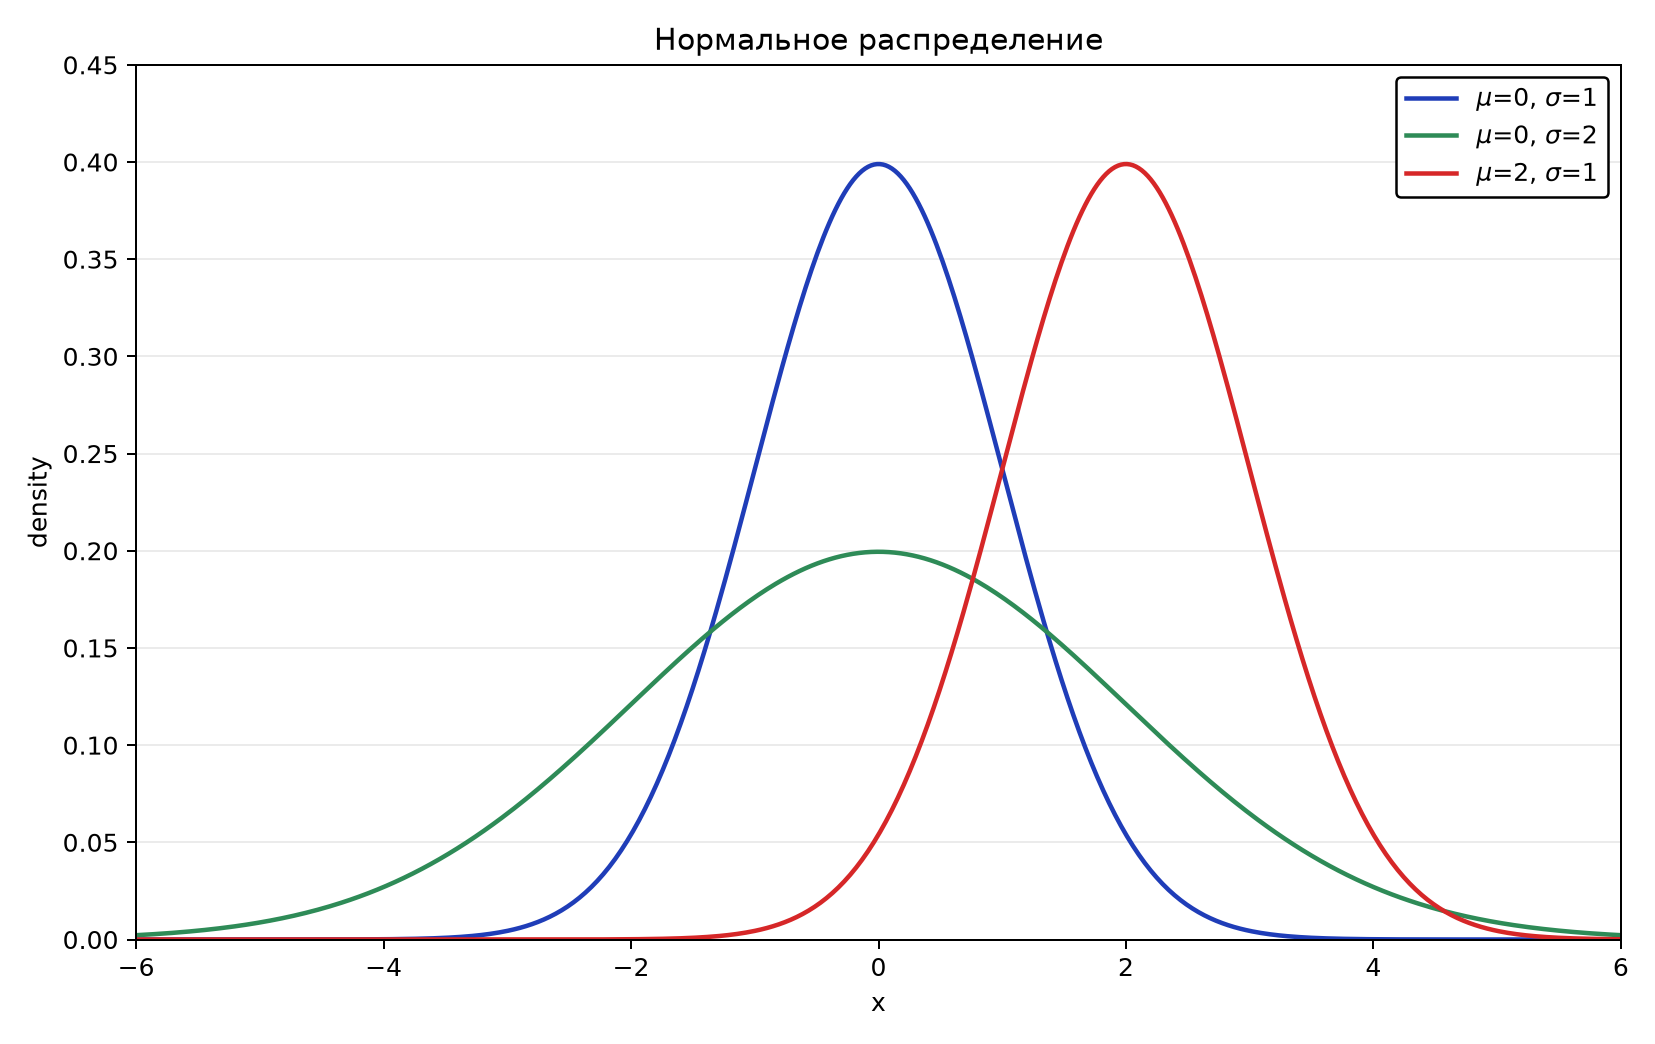
\includegraphics[keepaspectratio]{chapters/../assets/figures/normal_density_profiles.png}}

}

\caption{Примеры распределения Гаусса}

\end{figure}%

Из графика видно, что чем меньше \(\sigma\), тем уже распределение.

\subsection{Моменты распределения
Гуасса}\label{ux43cux43eux43cux435ux43dux442ux44b-ux440ux430ux441ux43fux440ux435ux434ux435ux43bux435ux43dux438ux44f-ux433ux443ux430ux441ux441ux430}

\begin{itemize}
\item
  \textbf{Математическое ожидание:} \(\mathbb{E}[X]=\mu\)
\item
  \textbf{Дисперсия:} \(Var(X)=\sigma^2\)
\end{itemize}

\subsubsection{\texorpdfstring{\textbf{Вывод}
\(\mathbb{E}[X]\)}{Вывод \textbackslash mathbb\{E\}{[}X{]}}}\label{ux432ux44bux432ux43eux434-mathbbex}

По определению:

\[\mathbb{E}[X]=\int_{-\infty}^\infty x\frac{1}{\sigma (2\pi)^{1/2}}\exp\left[-\frac{(x-\mu)^2}{2\sigma^2}\right]dx.\]

Перейдем к стандартной нормали:~\(z=(x−μ)/σ,~x=μ+σz,~dx=σdz:\)

\[\mathbb{E}[X]=\int_{-\infty}^\infty (\mu+\sigma z)\varphi(z)dz, \quad \varphi(z)=\frac{1}{\sqrt{2\pi}}e^{-z^2/2}.\]

\[\mathbb{E}[X]=\mu\int_{-\infty}^\infty \varphi(z)dz+\sigma\int_{-\infty}^\infty z\varphi(z)dz=\mu\cdot1+\sigma\cdot 0=\mu,\]

так как \(z\varphi(z)\) нечётная функция.

Итог:

\[\mathbb{E}[X]=\mu. \quad \blacksquare\]

\subsubsection{\texorpdfstring{\textbf{Вывод}
\(Var(X)\)}{Вывод Var(X)}}\label{ux432ux44bux432ux43eux434-varx}

По определению:

\[Var(X)=\mathbb{E}\left[(X-\mu)^2\right]=\int_{-\infty}^\infty (x-\mu)^2 f(x)dx.\]

Делая замену переменных \(z=(x-\mu)/\sigma,\) получим:

\[Var(X)=\sigma^2\int_{-\infty}^\infty z^2 \varphi(z) dz=\sigma^2 \mathbb{E}\left[Z^2\right], \quad Z\sim N(0,1),\]

где

\[\mathbb{E}\left[Z^2\right]=\int_{-\infty}^\infty z^2 \varphi(z)dz=\left[-z\varphi(z)\right]^{\infty}_{-\infty}+\int_{-\infty}^\infty \varphi(z)dz=1.\]

Итог:

\[Var(X)=\sigma^2. \quad \blacksquare\]

\section{Резюме по
распределениям}\label{ux440ux435ux437ux44eux43cux435-ux43fux43e-ux440ux430ux441ux43fux440ux435ux434ux435ux43bux435ux43dux438ux44fux43c}

{\def\LTcaptype{none} % do not increment counter
\begin{longtable}[]{@{}
  >{\centering\arraybackslash}p{(\linewidth - 6\tabcolsep) * \real{0.1926}}
  >{\centering\arraybackslash}p{(\linewidth - 6\tabcolsep) * \real{0.1037}}
  >{\centering\arraybackslash}p{(\linewidth - 6\tabcolsep) * \real{0.1111}}
  >{\centering\arraybackslash}p{(\linewidth - 6\tabcolsep) * \real{0.5778}}@{}}
\toprule\noalign{}
\begin{minipage}[b]{\linewidth}\centering
Название
\end{minipage} & \begin{minipage}[b]{\linewidth}\centering
Среднее
\end{minipage} & \begin{minipage}[b]{\linewidth}\centering
Дисперсия
\end{minipage} & \begin{minipage}[b]{\linewidth}\centering
Условия применения
\end{minipage} \\
\midrule\noalign{}
\endhead
\bottomrule\noalign{}
\endlastfoot
Биномиальное

\(K\sim Bin(n,p)\) & \(np\) & \(np(1-p)\) & Фиксированное \(n\);
независимые испытания; постоянное \(p\). \\
Пуассон

\(N\sim Pois(\lambda)\) & \(\lambda\) & \(\lambda\) & События в
фиксированном интервале; постоянная интенсивность; независимость. \\
Нормальное

\(X\sim N(\mu,\sigma)\) & \(\mu\) & \(\sigma^2\) & Непрерывные ошибки;
сумма многих малых независимых вкладов \\
\end{longtable}
}

\section{Итоги
главы}\label{ux438ux442ux43eux433ux438-ux433ux43bux430ux432ux44b-1}

\begin{itemize}
\tightlist
\item
  Данные в эксперименте флуктуируют, и эти флуктуации нужно описывать
  вероятностно.
\item
  Выбор распределения определяется физикой задачи.
\item
  Среднее и дисперсия --- первые количественные характеристики
  распределения.
\item
  Биномиальное, пуассоновское и нормальное распределения --- базовый
  рабочий набор экспериментатора.
\end{itemize}

Материалы курса:

\begin{itemize}
\tightlist
\item
  \href{https://neutrinohit.github.io/statistical-analysis-course/ru/slides/01_random_distributions.html}{Слайды
  лекции}
\item
  \href{https://neutrinohit.github.io/statistical-analysis-course/ru/slides/exercises/01_random_distributions_exercises.html}{Задачи}
\end{itemize}

\chapter{Характеристические функции и суммы случайных
величин}\label{ux445ux430ux440ux430ux43aux442ux435ux440ux438ux441ux442ux438ux447ux435ux441ux43aux438ux435-ux444ux443ux43dux43aux446ux438ux438-ux438-ux441ux443ux43cux43cux44b-ux441ux43bux443ux447ux430ux439ux43dux44bux445-ux432ux435ux43bux438ux447ux438ux43d}

{Статус главы}

Глава подготовлена как каркас по материалам третьей лекции. Полный
книжный текст, выводы и вычислительные примеры будут добавлены позднее.

\section{План
главы}\label{ux43fux43bux430ux43d-ux433ux43bux430ux432ux44b-1}

\begin{itemize}
\tightlist
\item
  распределение суммы случайных величин и свёртка;
\item
  характеристическая функция как преобразование Фурье;
\item
  независимость и произведение характеристических функций;
\item
  моменты, кумулянты и устойчивые распределения.
\end{itemize}

\section{Материалы
курса}\label{ux43cux430ux442ux435ux440ux438ux430ux43bux44b-ux43aux443ux440ux441ux430}

\begin{itemize}
\tightlist
\item
  \href{https://neutrinohit.github.io/statistical-analysis-course/ru/slides/02_characteristic_functions.html}{Слайды
  лекции}
\item
  \href{https://neutrinohit.github.io/statistical-analysis-course/ru/slides/exercises/02_characteristic_functions_exercises.html}{Задачи}
\end{itemize}

\chapter{Центральная предельная теорема и нормальное
распределение}\label{ux446ux435ux43dux442ux440ux430ux43bux44cux43dux430ux44f-ux43fux440ux435ux434ux435ux43bux44cux43dux430ux44f-ux442ux435ux43eux440ux435ux43cux430-ux438-ux43dux43eux440ux43cux430ux43bux44cux43dux43eux435-ux440ux430ux441ux43fux440ux435ux434ux435ux43bux435ux43dux438ux435}

{Статус главы}

Глава подготовлена как каркас по материалам четвёртой лекции. Полный
текст, доказательства и интерактивы будут добавлены позднее.

\section{План
главы}\label{ux43fux43bux430ux43d-ux433ux43bux430ux432ux44b-2}

\begin{itemize}
\tightlist
\item
  центральная предельная теорема и её условия;
\item
  стандартное нормальное распределение и квантили;
\item
  стандартизация случайных величин;
\item
  проверка совместимости двух измерений.
\end{itemize}

\section{Материалы
курса}\label{ux43cux430ux442ux435ux440ux438ux430ux43bux44b-ux43aux443ux440ux441ux430-1}

\begin{itemize}
\tightlist
\item
  \href{https://neutrinohit.github.io/statistical-analysis-course/ru/slides/03_central_limit_theorem.html}{Слайды
  лекции}
\item
  \href{https://neutrinohit.github.io/statistical-analysis-course/ru/slides/exercises/03_central_limit_theorem_exercises.html}{Задачи}
\end{itemize}

\chapter{Когда не возникает гауссового
распределения}\label{ux43aux43eux433ux434ux430-ux43dux435-ux432ux43eux437ux43dux438ux43aux430ux435ux442-ux433ux430ux443ux441ux441ux43eux432ux43eux433ux43e-ux440ux430ux441ux43fux440ux435ux434ux435ux43bux435ux43dux438ux44f}

{Статус главы}

Глава подготовлена как каркас по материалам пятой лекции. Полный текст и
практические примеры будут добавлены позднее.

\section{План
главы}\label{ux43fux43bux430ux43d-ux433ux43bux430ux432ux44b-3}

\begin{itemize}
\tightlist
\item
  тяжёлые хвосты и отсутствие конечной дисперсии;
\item
  корреляции и нарушение независимости;
\item
  смеси распределений, пороги и отбор;
\item
  малые счёты и диагностика негауссовости.
\end{itemize}

\section{Материалы
курса}\label{ux43cux430ux442ux435ux440ux438ux430ux43bux44b-ux43aux443ux440ux441ux430-2}

\begin{itemize}
\tightlist
\item
  \href{https://neutrinohit.github.io/statistical-analysis-course/ru/slides/04_non_gaussian_clt_violations.html}{Слайды
  лекции}
\item
  \href{https://neutrinohit.github.io/statistical-analysis-course/ru/slides/exercises/04_non_gaussian_clt_violations_exercises.html}{Задачи}
\end{itemize}

\part{II. Моделирование и оценивание}

\chapter{Распространение ошибок, ковариации и многомерный
гаусс}\label{ux440ux430ux441ux43fux440ux43eux441ux442ux440ux430ux43dux435ux43dux438ux435-ux43eux448ux438ux431ux43eux43a-ux43aux43eux432ux430ux440ux438ux430ux446ux438ux438-ux438-ux43cux43dux43eux433ux43eux43cux435ux440ux43dux44bux439-ux433ux430ux443ux441ux441}

{Статус главы}

Глава подготовлена как каркас по материалам шестой лекции. Полный текст,
физические примеры и интерактивы будут добавлены позднее.

\section{План
главы}\label{ux43fux43bux430ux43d-ux433ux43bux430ux432ux44b-4}

\begin{itemize}
\tightlist
\item
  линейное распространение неопределённостей;
\item
  ковариации и коэффициенты корреляции;
\item
  ковариационная матрица;
\item
  двумерный гаусс, контуры и вероятностные эллипсы.
\end{itemize}

\section{Материалы
курса}\label{ux43cux430ux442ux435ux440ux438ux430ux43bux44b-ux43aux443ux440ux441ux430-3}

\begin{itemize}
\tightlist
\item
  \href{https://neutrinohit.github.io/statistical-analysis-course/ru/slides/05_error_propagation_and_covariance.html}{Слайды
  лекции}
\item
  \href{https://neutrinohit.github.io/statistical-analysis-course/ru/slides/exercises/05_error_propagation_and_covariance_exercises.html}{Задачи}
\end{itemize}

\chapter{Метод Монте-Карло и
псевдоэксперименты}\label{ux43cux435ux442ux43eux434-ux43cux43eux43dux442ux435-ux43aux430ux440ux43bux43e-ux438-ux43fux441ux435ux432ux434ux43eux44dux43aux441ux43fux435ux440ux438ux43cux435ux43dux442ux44b}

{Статус главы}

Глава подготовлена как каркас по материалам седьмой лекции. Полный
текст, алгоритмы и воспроизводимые примеры будут добавлены позднее.

\section{План
главы}\label{ux43fux43bux430ux43d-ux433ux43bux430ux432ux44b-5}

\begin{itemize}
\tightlist
\item
  генерация случайных величин;
\item
  интегрирование методом Монте-Карло;
\item
  псевдоэксперименты и распространение неопределённостей;
\item
  моделирование отклика эксперимента.
\end{itemize}

\section{Материалы
курса}\label{ux43cux430ux442ux435ux440ux438ux430ux43bux44b-ux43aux443ux440ux441ux430-4}

\begin{itemize}
\tightlist
\item
  \href{https://neutrinohit.github.io/statistical-analysis-course/ru/slides/06_monte_carlo_method.html}{Слайды
  лекции}
\item
  \href{https://neutrinohit.github.io/statistical-analysis-course/ru/slides/exercises/06_monte_carlo_method_exercises.html}{Задачи}
\end{itemize}

\chapter{Оценивание параметров и метод максимального
правдоподобия}\label{ux43eux446ux435ux43dux438ux432ux430ux43dux438ux435-ux43fux430ux440ux430ux43cux435ux442ux440ux43eux432-ux438-ux43cux435ux442ux43eux434-ux43cux430ux43aux441ux438ux43cux430ux43bux44cux43dux43eux433ux43e-ux43fux440ux430ux432ux434ux43eux43fux43eux434ux43eux431ux438ux44f}

{Статус главы}

Глава подготовлена как каркас по материалам восьмой лекции. Полный
текст, выводы и примеры оценивания будут добавлены позднее.

\section{План
главы}\label{ux43fux43bux430ux43d-ux433ux43bux430ux432ux44b-6}

\begin{itemize}
\tightlist
\item
  оценки и их свойства;
\item
  функция и метод максимального правдоподобия;
\item
  информация Фишера и точность оценки;
\item
  профильное правдоподобие и диагностика фита.
\end{itemize}

\section{Материалы
курса}\label{ux43cux430ux442ux435ux440ux438ux430ux43bux44b-ux43aux443ux440ux441ux430-5}

\begin{itemize}
\tightlist
\item
  \href{https://neutrinohit.github.io/statistical-analysis-course/ru/slides/07_parameter_estimation_and_maximum_likelihood.html}{Слайды
  лекции}
\item
  \href{https://neutrinohit.github.io/statistical-analysis-course/ru/slides/exercises/07_parameter_estimation_and_maximum_likelihood_exercises.html}{Задачи}
\end{itemize}

\chapter{Метод наименьших
квадратов}\label{ux43cux435ux442ux43eux434-ux43dux430ux438ux43cux435ux43dux44cux448ux438ux445-ux43aux432ux430ux434ux440ux430ux442ux43eux432}

{Статус главы}

Глава подготовлена как каркас по материалам девятой лекции. Полный
текст, вычислительные примеры и интерактивы будут добавлены позднее.

\section{План
главы}\label{ux43fux43bux430ux43d-ux433ux43bux430ux432ux44b-7}

\begin{itemize}
\tightlist
\item
  связь метода наименьших квадратов с гауссовским правдоподобием;
\item
  линейные и нелинейные модели;
\item
  коррелированные неопределённости;
\item
  остатки и качество подгонки.
\end{itemize}

\section{Материалы
курса}\label{ux43cux430ux442ux435ux440ux438ux430ux43bux44b-ux43aux443ux440ux441ux430-6}

\begin{itemize}
\tightlist
\item
  \href{https://neutrinohit.github.io/statistical-analysis-course/ru/slides/08_method_of_least_squares.html}{Слайды
  лекции}
\item
  \href{https://neutrinohit.github.io/statistical-analysis-course/ru/slides/exercises/08_method_of_least_squares_exercises.html}{Задачи}
\end{itemize}

\part{III. Статистический вывод}

\chapter{Статистические тесты: общие
понятия}\label{ux441ux442ux430ux442ux438ux441ux442ux438ux447ux435ux441ux43aux438ux435-ux442ux435ux441ux442ux44b-ux43eux431ux449ux438ux435-ux43fux43eux43dux44fux442ux438ux44f}

{Статус главы}

Глава подготовлена как каркас по материалам десятой лекции. Полный
текст, примеры и интерактивные тесты будут добавлены позднее.

\section{План
главы}\label{ux43fux43bux430ux43d-ux433ux43bux430ux432ux44b-8}

\begin{itemize}
\tightlist
\item
  нулевая и альтернативная гипотезы;
\item
  ошибки первого и второго рода;
\item
  мощность и критическая область;
\item
  статистика теста и \(p\)-value.
\end{itemize}

\section{Материалы
курса}\label{ux43cux430ux442ux435ux440ux438ux430ux43bux44b-ux43aux443ux440ux441ux430-7}

\begin{itemize}
\tightlist
\item
  \href{https://neutrinohit.github.io/statistical-analysis-course/ru/slides/09_statistical_tests_basics.html}{Слайды
  лекции}
\item
  \href{https://neutrinohit.github.io/statistical-analysis-course/ru/slides/exercises/09_statistical_tests_basics_exercises.html}{Задачи}
\end{itemize}

\chapter{Статистики тестов и многомерные
методы}\label{ux441ux442ux430ux442ux438ux441ux442ux438ux43aux438-ux442ux435ux441ux442ux43eux432-ux438-ux43cux43dux43eux433ux43eux43cux435ux440ux43dux44bux435-ux43cux435ux442ux43eux434ux44b}

{Статус главы}

Глава подготовлена как каркас по материалам одиннадцатой лекции. Полный
текст, примеры и практические рекомендации будут добавлены позднее.

\section{План
главы}\label{ux43fux43bux430ux43d-ux433ux43bux430ux432ux44b-9}

\begin{itemize}
\tightlist
\item
  отношение правдоподобий и профильные статистики;
\item
  асимптотические распределения;
\item
  многомерные дискриминанты и ROC-кривые;
\item
  переобучение, калибровка и валидация.
\end{itemize}

\section{Материалы
курса}\label{ux43cux430ux442ux435ux440ux438ux430ux43bux44b-ux43aux443ux440ux441ux430-8}

\begin{itemize}
\tightlist
\item
  \href{https://neutrinohit.github.io/statistical-analysis-course/ru/slides/10_test_statistics_and_multivariate_methods.html}{Слайды
  лекции}
\item
  \href{https://neutrinohit.github.io/statistical-analysis-course/ru/slides/exercises/10_test_statistics_and_multivariate_methods_exercises.html}{Задачи}
\end{itemize}

\chapter{Проверка согласия и статистическая
значимость}\label{ux43fux440ux43eux432ux435ux440ux43aux430-ux441ux43eux433ux43bux430ux441ux438ux44f-ux438-ux441ux442ux430ux442ux438ux441ux442ux438ux447ux435ux441ux43aux430ux44f-ux437ux43dux430ux447ux438ux43cux43eux441ux442ux44c}

{Статус главы}

Глава подготовлена как каркас по материалам двенадцатой лекции. Полный
текст, примеры и интерактивы будут добавлены позднее.

\section{План
главы}\label{ux43fux43bux430ux43d-ux433ux43bux430ux432ux44b-10}

\begin{itemize}
\tightlist
\item
  критерии согласия и анализ остатков;
\item
  статистики Пирсона и deviance;
\item
  калибровка \(p\)-value;
\item
  локальная, глобальная значимость и look-elsewhere effect.
\end{itemize}

\section{Материалы
курса}\label{ux43cux430ux442ux435ux440ux438ux430ux43bux44b-ux43aux443ux440ux441ux430-9}

\begin{itemize}
\tightlist
\item
  \href{https://neutrinohit.github.io/statistical-analysis-course/ru/slides/11_goodness_of_fit_and_significance.html}{Слайды
  лекции}
\item
  \href{https://neutrinohit.github.io/statistical-analysis-course/ru/slides/exercises/11_goodness_of_fit_and_significance_exercises.html}{Задачи}
\end{itemize}

\chapter{Фельдман--Казинс, CLs и родственные
методы}\label{ux444ux435ux43bux44cux434ux43cux430ux43dux43aux430ux437ux438ux43dux441-cls-ux438-ux440ux43eux434ux441ux442ux432ux435ux43dux43dux44bux435-ux43cux435ux442ux43eux434ux44b}

{Статус главы}

Глава подготовлена как каркас по материалам тринадцатой лекции. Полный
текст, численные построения и примеры будут добавлены позднее.

\section{План
главы}\label{ux43fux43bux430ux43d-ux433ux43bux430ux432ux44b-11}

\begin{itemize}
\tightlist
\item
  построение Неймана и покрытие;
\item
  правила упорядочивания;
\item
  unified intervals Фельдмана--Казинса;
\item
  метод \(CL_s\) и ожидаемые ограничения.
\end{itemize}

\section{Материалы
курса}\label{ux43cux430ux442ux435ux440ux438ux430ux43bux44b-ux43aux443ux440ux441ux430-10}

\begin{itemize}
\tightlist
\item
  \href{https://neutrinohit.github.io/statistical-analysis-course/ru/slides/12_feldman_cousins_and_cls.html}{Слайды
  лекции}
\item
  \href{https://neutrinohit.github.io/statistical-analysis-course/ru/slides/exercises/12_feldman_cousins_and_cls_exercises.html}{Задачи}
\end{itemize}

\chapter{Интервальные оценки и установление
ограничений}\label{ux438ux43dux442ux435ux440ux432ux430ux43bux44cux43dux44bux435-ux43eux446ux435ux43dux43aux438-ux438-ux443ux441ux442ux430ux43dux43eux432ux43bux435ux43dux438ux435-ux43eux433ux440ux430ux43dux438ux447ux435ux43dux438ux439}

{Статус главы}

Глава подготовлена как каркас по материалам четырнадцатой лекции. Полный
текст, сравнение процедур и вычислительные примеры будут добавлены
позднее.

\section{План
главы}\label{ux43fux43bux430ux43d-ux433ux43bux430ux432ux44b-12}

\begin{itemize}
\tightlist
\item
  pivotal quantities и классические интервалы;
\item
  интервалы Вальда и Уилсона;
\item
  profile likelihood и многомерные контуры;
\item
  bootstrap, односторонние ограничения и coverage.
\end{itemize}

\section{Материалы
курса}\label{ux43cux430ux442ux435ux440ux438ux430ux43bux44b-ux43aux443ux440ux441ux430-11}

\begin{itemize}
\tightlist
\item
  \href{https://neutrinohit.github.io/statistical-analysis-course/ru/slides/13_interval_estimation_and_limits.html}{Слайды
  лекции}
\item
  \href{https://neutrinohit.github.io/statistical-analysis-course/ru/slides/exercises/13_interval_estimation_and_limits_exercises.html}{Задачи}
\end{itemize}

\part{IV. Неопределённости и альтернативный вывод}

\chapter{Nuisance-параметры и систематические
неопределённости}\label{nuisance-ux43fux430ux440ux430ux43cux435ux442ux440ux44b-ux438-ux441ux438ux441ux442ux435ux43cux430ux442ux438ux447ux435ux441ux43aux438ux435-ux43dux435ux43eux43fux440ux435ux434ux435ux43bux451ux43dux43dux43eux441ux442ux438}

{Статус главы}

Глава подготовлена как каркас по материалам пятнадцатой лекции. Полный
текст, практические модели и примеры будут добавлены позднее.

\section{План
главы}\label{ux43fux43bux430ux43d-ux433ux43bux430ux432ux44b-13}

\begin{itemize}
\tightlist
\item
  nuisance-параметры и constrained likelihood;
\item
  ковариационные модели систематик;
\item
  профилирование и маргинализация;
\item
  влияние систематических неопределённостей на результат.
\end{itemize}

\section{Материалы
курса}\label{ux43cux430ux442ux435ux440ux438ux430ux43bux44b-ux43aux443ux440ux441ux430-12}

\begin{itemize}
\tightlist
\item
  \href{https://neutrinohit.github.io/statistical-analysis-course/ru/slides/14_nuisance_parameters_and_systematics.html}{Слайды
  лекции}
\item
  \href{https://neutrinohit.github.io/statistical-analysis-course/ru/slides/exercises/14_nuisance_parameters_and_systematics_exercises.html}{Задачи}
\end{itemize}

\chapter{Байесовский вывод и практические
примеры}\label{ux431ux430ux439ux435ux441ux43eux432ux441ux43aux438ux439-ux432ux44bux432ux43eux434-ux438-ux43fux440ux430ux43aux442ux438ux447ux435ux441ux43aux438ux435-ux43fux440ux438ux43cux435ux440ux44b}

{Статус главы}

Глава подготовлена как каркас по материалам шестнадцатой лекции. Полный
текст, вычислительные примеры и сравнение подходов будут добавлены
позднее.

\section{План
главы}\label{ux43fux43bux430ux43d-ux433ux43bux430ux432ux44b-14}

\begin{itemize}
\tightlist
\item
  теорема Байеса и апостериорное распределение;
\item
  выбор априорного распределения;
\item
  credible intervals и предсказательные распределения;
\item
  практические примеры и сравнение с частотным выводом.
\end{itemize}

\section{Материалы
курса}\label{ux43cux430ux442ux435ux440ux438ux430ux43bux44b-ux43aux443ux440ux441ux430-13}

\begin{itemize}
\tightlist
\item
  \href{https://neutrinohit.github.io/statistical-analysis-course/ru/slides/15_bayesian_examples.html}{Слайды
  лекции}
\item
  \href{https://neutrinohit.github.io/statistical-analysis-course/ru/slides/exercises/15_bayesian_examples_exercises.html}{Задачи}
\end{itemize}


\backmatter


\end{document}
